%%==================================================
%% diss.tex for SJTU Bachelor Thesis
%% based on CASthesis
%% version: 0.3a
%% Encoding: UTF-8
%%==================================================

% 字号选项: c5size 五号(默认) cs4size 小四
% 双面打印(注意字号设置)
%\documentclass[cs4size, a4paper, twoside]{sjtuthesis} 
% 单面打印(注意字号设置)
\documentclass[cs4size, a4paer, oneside, openany, nocap]{sjtuthesis} 

\CTEXsetup[aftername={\nobreak\quad}]{chapter}
\CTEXsetup[format={\centering}]{chapter}

%% My changes below
\usepackage[ruled,linesnumbered,boxed]{algorithm2e}
\usepackage{tabularx}

\usepackage{titlesec} 
              
%\def\CTEX@chapter@beforeskip{1\p@}
%\def\CTEX@chapter@afterskip{12\p@}
\renewcommand{\figurename}{Figure}  
\renewcommand{\tablename}{Table}
\renewcommand{\bibname}{REFERENCES}

%% My changes above

% \usepackage[sectionbib]{chapterbib}%每章都用参考文献
\usepackage{setspace}
\newboolean{DOIT}
\setboolean{DOIT}{false}%编译某些只想自己看的内容,编译true,否则false

%% 行距缩放因子(x倍字号)
\renewcommand{\baselinestretch}{1.3}

% 设置图形文件的搜索路径
\graphicspath{{figure/}{figures/}{logo/}{logos/}{graph/}{graphs}}

%%========================================
%% 在sjtuthesis.cls中定义的有用命令
%%========================================
% \cndash 中文破折号
% 数学常量
% \me 对数常数e
% \mi 虚数单位i
% \mj 虚数单位j
% \dif 直立的微分算符d为直立体。
% 可伸长的数学箭头、等号
% \myRightarrow{}{}
% \myLeftarrow{}{}
% \myBioarrow{}{}
% \myLongEqual{}{}
% 参考文献
% \upcite{} 上标引用
%%========================================


\begin{document}

%%%%%%%%%%%%%%%%%%%%%%%%%%%%%% 
%% 封面
%%%%%%%%%%%%%%%%%%%%%%%%%%%%%% 

% 中文封面内容(关注内容而不是形式)
\title{基于OpenFlow的数据中心监控负载均衡问题}
\author{陈宇翔}
\advisor{高晓沨}
\degree{学士}
\school{上海交通大学}
\institute{电子信息与电气工程学院}
\studentnumber{5110309783}
\major{电子信息科学类}

% 英文封面内容(关注内容而不是表现形式)
\englishtitle{Load balancing in Data Center Networks based on OpenFlow}
\englishauthor{Yuxiang Chen}
\englishadvisor{Prof. Xiaofeng Gao}
\englishschool{Shanghai Jiao Tong University}
\englishinstitute{Depart of Computer Science and Engineering \\
  Shanghai Jiao Tong University \\
  Shanghai, P.R.China}
\englishdegree{Bachelor}
\englishmajor{Computer Science}
\englishdate{May. 16th, 2015}

% 封面
\maketitle

% 英文封面
\makeenglishtitle

% 论文原创性声明和使用授权
\makeDeclareOriginal
\makeDeclareAuthorization

%%%%%%%%%%%%%%%%%%%%%%%%%%%%%% 
%% 前言
%%%%%%%%%%%%%%%%%%%%%%%%%%%%%% 
\frontmatter
\fancypagestyle{plain}{% 设置开章页页眉页脚风格(只有页码作为页脚)
  \fancyhf{}%
  \fancyhead[L]{\small {\it 
\includegraphics[width=0.22\textwidth]{sjtubanner}}}  % 奇数页左页眉
  \fancyhead[R]{\small {\it Load balancing in Data Center Networks based on OpenFlow}}                   % 奇数页右页眉
  \fancyfoot[C]{--- {\bf\thepage} ---}      % 页脚
}

% 摘要
%%==================================================
%% abstract.tex for SJTU Bachelor Thesis
%% version: 0.5.2
%% Encoding: UTF-8
%%==================================================
\pagestyle{frontmatter}

\begin{abstract}

	软件定义网络(Software Defined Network, SDN)是近几年来在计算机网络领域兴起的概念,其主要目标是通过对网络的控制和管理进行精简,来利用网络的可编程性,达到促进网络优化的目的。SDN作为一种新的网络模式,可以将硬件的功能进行划分,把执行数据包转发的部分从硬件的控制决策部分中分离出来。这种对控制逻辑的分离,将以前集成在硬件中的控制部分抽象成一个由软件定义的控制器,从而使得整个网络的配置更加灵活。

	从整体结构上来看,SDN中的控制功能(控制平面)被集中到了一个基于软件的控制器,而网络中的硬件设备则主要用于实现数据包的转发(数据平面)。要使得数据平面和控制平面可以进行沟通,就需要一个可编程的接口对这两部分进行连接,OpenFlow则是由斯坦福大学提出的用于SDN的一个接口的实现。

	而数据中心网络(Data Center Network, DCN)则是一个更加广为人知的概念。在当今的网络形势下,越来越多的公司致力于提供云端服务,这就必然涉及到提供云服务的数据中心中的负载均衡问题。而我们这篇文章则将数据中心的负载均衡定义在OpenFlow的框架下,提供一种在SDN环境下提高DCN性能的解决方案。

	一个一般的SDN网络主要由控制器(controller),交换机(switch)和主机(host)组成,每个交换机可以控制若干个主机,每个控制器也可以控制若干个交换机。由于主机之间要不停地进行通信,因此会在整个网络中产生流量。因此,交换机需要对这些网络流量(数据包)进行转发。由于每个交换机转发的流量不同,因此也会有不同的负载。而在每个交换机之上,还有控制器对交换机的流量进行转发。对于目前较为普遍的SDN网络,整个网络中一般由一个集中式的控制器来控制所有交换机的转发逻辑,而这个唯一的控制器在大型网络中将很可能成为整个网络的瓶颈。

	在最近的文献中,可以看到,很多学者致力于对分布式控制器的研究,并提出了在DCN中部署多个控制器的想法。在一个可以实现OpenFlow协议的网络中部署多个控制器,可以有效地将不同交换机的控制交给不同的控制器,从而尽量消除唯一的控制器成为瓶颈的可能性。但是如果只是随机地将交换机分配给控制器,或者是通过某种初始化算法分配后一直维持控制器和交换机的对应关系,则可能会因为网络中的流量变化而导致控制器间的负载出现不均衡,从而造成网络的局部瓶颈,影响整个网络的性能。

	因此,提供一种在网络状态变化时可以动态迁移交换机的方法是十分必要的。通过将交换机从负载较重的控制器迁移到负载相对较轻的控制器中,可以对控制器的负载实现平衡。为了解决这一问题,本文首先建立了在能实现OpenFlow协议的DCN网络中多控制器和多交换机的负载均衡模型,同时借鉴前人在数据中心中部署多个控制器来控制网络流量的算法,来设计适用于OpenFlow框架的多控制器负载均衡算法,并通过仿真实验来验证负载均衡算法在网络中的有效性。

	上述算法的主要原理是通过收集网络中交换机的负载信息,来计算每个控制器的平均负载,然后将超过平均负载的控制器所管理的交换机向未超过负载的控制器进行迁移,从而使控制器的负载达到均衡的状态。但是在实际的网络中,这种负载均衡方法存在着很多的局限性。实际上,每个控制器由于自身性能的局限性,可以处理的负载是有其上限的,因此本文又提出了一种改进的算法。通过计算网络中的当前流量,同时计算所有可用控制器的性能上限,来计算控制器可用性能的平均百分比,并以此分配每个控制器的“平均”容量。这种方法通过计算平均性能百分比,使得所有的控制器都会处在相对均衡的状态进行工作,依照其处理能力的不同而执行不同的任务量。

	除此之外,在一个大型分布式网络中,控制器和交换机可能分布在任何地方。也就是说,控制器之间可以相隔很远,而控制器与其可以控制的交换机之间也可能相隔很远。在这种情况下,如果将交换机的控制权交给与它相对较近的控制器无疑会提高网络流的处理速度,进而提高网络的性能。因此,本文同时也提出了用于有不同优先级(权值)的交换机的迁移算法,通过以交换机的权值为最优先标准,来对控制器的负载进行均衡。

	通过对上述算法进行实现并进行仿真实验,我们验证了算法的有效性与在SDN网络中部署这些算法的可能性,从而为大型SDN网络的负载均衡提供了可能的实现方案。

  \keywords{负载均衡,多控制器,软件定义网络,负载上限}
\end{abstract}

\begin{englishabstract}

Software Defined Network (SDN) is a concept in the area of computer network, which becomes very popular recent years. The main purpose of SDN is to simplify the control and management of the network, thus making use of the programming ability of SDN. As a new pattern of computer network, SDN can divide the function of the hardware into two parts, i.e., taking the part that forwards data packets out of the control desicion part. By spliting up the two functions, the controller part which used to be integrated in hardware now become a software-defined controller, which makes the configuration of the whole network more flexible.

Viewing the structure as a whole, the control function control plane) is centralized as a software defined controller, and the hardware devices are mainly used in implementing the forwarding of data packets (data plane). In order to connect these two planes, a set of application programming interface (API) is needed, and OpenFlow is a realization of this kind of API in SDN, raising by Stanford University.

And Data Center Network (DCN) is a more popular concept. In current network situation, more and more companies aim at providing customers with cloud services, which will certainly involve the problem of load balancing in a data center. And in this paper, we will provide a practical scheme to be used in SDN environment, in order to improve the performance of a DCN that is defined under the OpenFlow structure.

A general SDN network is mainly composed of controller, switch and host. A switch can control several hosts, and a controller can control several switches. As a result of the lasting communication among all the hosts, traffic will be generated in the network. And the switches have to forward these packets. Since each host generates different amount of traffic, each switch may have different load. In the kind of SDN that is very popular nowadays, a central controller is usually used to take control of the forwarding schemes of all switches. However, this only controller is very likely to become the bottleneck in a very large network.

From recent publications, we can see that many scholars are engaged in the research of devolved controllers, and come up with the idea of deploying multiple controllers in DCN. In a network that implements the OpenFlow protocols, deploying multiple controllers can help the effectively migration of switches between two controllers, and thus avoid the situation of a central overloaded controller. However, if we just randomly distribute switches to controllers, or keep the mapping of controllers and switches unchanged after initialization, then as a result of traffic changing over time, the load among all controllers may become unbalanced, giving rise to local bottlenecks in the network, and decreasing the performance of the network.

Thus, it is very necessary to come up with a method that can dynamically migrate the switches according to current network conditions. By migrate the switches from overloaded controllers to controllers that have comparatively less load, we can balance the load in the whole network. To solve this problem, this paper first establishes a model of multiple controllers and multiple switches in a software defined network that implements OpenFlow protocol, and then refer to the load balancing algorithms of several controllers raised in Data Center Networks to design an algorithm, that can be used in OpenFlow structure for load balancing of multiple controllers. Then we use simulation to prove the effectiveness of this algorithm.

The main idea of the above algorithm is to collect the load information of switches and controllers in the network, and calculate the average load that should be allocated to each controller. Then for those controllers that exceed the average load, we have to migrate the switches that are controlled by these controllers, to the controllers that are under the average level, and thus trying to balance the load in the network. However, in actual networks, the method have some limits. In fact, each controller can only process a limited load not exceeding its ability. Thus this paper raised another improved algorithm to solve this problem. By calculating the current traffic in the network and the maximal load that can be processed by all controllers in the network, we can get a percentage, which implicates the adequate amount of traffic that a controller should take. And then with this percentage, we can calculate the real 'average' of each controller, and migrate the switches according to this value. This method makes use of this percentage, and make all the controllers working in a comparatively balanced condition -- processing different load refering to its maximal ability.

Apart from this, in a large distributed network, controllers and switches can be placed in any places. That is to say, there may be a very long distance between the controllers, and there may also be a very long distance between the switches and its potential/real(slave/master) controllers. In this condition, if we give the control power of a certain switch to the controller that is near to it, it will certainly help increase the processing speed of traffic, and thus improve the performance of this network. Thus, we also raise an migration algorithm that take the priority (weight) of each switch into consideration. By give the highest priority to the weight of switches, we balance the load of the whole network. 

By implementing all above algorthms and doing simulations, we prove the effectiveness of the algorithms and the possibity of deploying these algorithms in real software defined networks,thus bringing up with possible schemes of load balancing in large SDN.

  \englishkeywords{\large Load Balancing, Limited Ability, Multiple Controllers, Software Defined Network, OpenFlow}
  
\end{englishabstract}


% 目录
\tableofcontents
% 表格索引
\listoftables
% 插图索引
\listoffigures

% \addcontentsline{toc}{chapter}{\listfigurename} %将表格索引加入全文目录
% \addcontentsline{toc}{chapter}{\listtablename}  %将图索引加入全文目录

% 主要符号、缩略词对照表
% %%==================================================
%% symbol.tex for SJTU Bachelor Thesis
%% version: 0.5.2
%% Encoding: UTF-8
%%==================================================

\chapter{主要符号对照表}
\label{chap:symb}
\begin{tabular}{ll}

 \hspace{2em}$\epsilon$       & \hspace{5em}介电常数 \\
 \hspace{2em}$\mu$ \qquad     & \hspace{5em}磁导率 \\
  \hspace{2em}$\epsilon$       & \hspace{5em}介电常数 \\
 \hspace{2em}$\mu$ \qquad     & \hspace{5em}磁导率 \\
 \hspace{2em}$\epsilon$       & \hspace{5em}介电常数 \\
 \hspace{2em}$\mu$ \qquad     & \hspace{5em}磁导率 \\
 \hspace{2em}$\epsilon$       & \hspace{5em}介电常数 \\
 \hspace{2em}$\mu$ \qquad     & \hspace{5em}磁导率 \\


\end{tabular}


%%%%%%%%%%%%%%%%%%%%%%%%%%%%%% 
%% 正文
%%%%%%%%%%%%%%%%%%%%%%%%%%%%%% 

\mainmatter
\fancypagestyle{plain}{% 设置开章页页眉页脚风格(只有页码作为页脚)
  \fancyhf{}%
  \fancyhead[L]{\small {\it 
\includegraphics[width=0.22\textwidth]{sjtubanner}}}  % 奇数页左页眉
  \fancyhead[R]{\small {\it Load balancing in Data Center Networks based on OpenFlow}}                   % 奇数页右页眉
  %\fancyfoot[C]{\small ~{\bf\thepage}~~{\bf of}~~{\bf\pageref{lastpage}}~}      % 页脚
  \fancyfoot[C]{\small ~{\bf\thepage}~~{\bf of~~68}~}      % 页脚
  %\fancyfoot[C]{\small ~{\bf\thepage}~}      % 页脚
}
\pagestyle{plain}

%% 各章正文内容
%%==========================
%% chapter01.tex for SJTU Bachelor Thesis
%% version: 0.5.2
%% Encoding: UTF-8
%%==================================================

%\bibliographystyle{sjtu2} %[此处用于每章都生产参考文献]
\pagestyle{plain}
\renewcommand{\chaptername}{Chapter \CJKnumber{\thechapter}}

\chapter{Introduction}
\label{chap:intro}

Currently, the structure and function of the Internet has become more and more complex, as a result of the rapid expansion of the Internet scale. Meanwhile, the hardwares in the network are given more and more responsiblities. For example, the router, which should have been a simple data forwarding unit, has now taken control of filtering packets, distinguishing services, and deciding the quality of service. However, the coupling of logical controlling and data forwarding on the hardware makes it very hard to manage the control plane of the Internet, and thus hindering the deployment of new flexible structures and techologies.

To solve this problem existed in the widely used Internet structure, several projects have been raised, such as Global Environment for Network Innovations (GENI) \cite{geni} of US, Future Internet Research and Experimentation Initative (FIRE) \cite{fire} of EU, AKARI \& JGN2plus \cite{akari} of Japan, and Smart Applications on Virtual Infrastructure (SAVI) \cite{savi} of Canada. They all aim at exploring new Internet structures, so that researchers are allowed to test their ideas on a virtualized network. Among all these kinds of projects, though not born for network virtualization on purpose, OpenFlow \cite{openflow} brings endless posibilities on the development of future network.

OpenFlow has its spring in Clean State Project Team of Stanford University. The final purpose of the Clean State program is to reinvent the Internet, aiming at changing the basic structure of the current network, which is out-of-date and is hard to develop. Martin Casado, a student of Stanford, lead the project Ethane \cite{ethane} which is related to network security and management in 2006. The project attempted to allow network administrator to design flow-based safety control policies conveniently, and apply these security policies to various network devices, so that researchers can realize the safety control of the whole network, by using a centralized controller. Shortly afterwards, inspired by Ethane and its predeccessor SANE \cite{sane}, Martin and his supervisor found that the design of Ethane can be generalized. By separating the control plane and data plane, and using standard application programming interface of a centralized controller to configure and manage the network devices, it is possible to make the design and management of the network more flexible, and promote the development of Internet. Thus the concept of OpenFlow was raised, and was introduced in detail in the paper -- OpenFlow: Enabling Innovation in Campus Networks \cite{openflow}, published on SIGCOMM, 2008. 

Apart from elaborating the operational principle of OpenFlow, the paper also listed several applicable situations of OpenFlow. Then later Nick and his team put forward the concept of Software Defined Network (SDN), based on the programmable character OpenFlow brings to the network. If all the devices in the network can be regarded as managable resources, then it is possible to abstract a network operating system (OS) according to the principle of OS. Then users can develop various applications on this platform, and satisfy different requirements of network resources by defining logical network topology, without caring about the physical topology.

In fact, though OpenFlow and SDN drew a great deal of attention in the industry after they are published, the idea of programmable network and separating the control plane and data plane can be traced far to the past. In 1995, a serious of activities were launched by the open Signaling Working Group (OPENSIG), trying to make the Internet more flexible and easier to program. Later, Active Network first came up with the idea of programmable network basic devices, which was intended to be used in custom services. Then the project team of forwarding and control element separation (ForCES) divides the network element to control element and forwarding element, based on programmable network structure. Though the inside structure was redefined in this way, the control element and the forwarding element were still presented as a single network unit. To solve the problem that the control plane and the devices are in a tight coupling, Greenberg and his assistants redesigned the control and management structure of the Internet, and raised a new system structure called 4D (decision, dissemination, discovery, data) \cite{4d1, 4d2} . Under the 4D structure, these four function planes are separated, and make the management of the network clean and clear. In fact, SANE, the predecessor of Ethane, also used 4D structure as its designing principle.

Briefly speaking, OpenFlow is in fact a kind of communication protocol between controllers and switches \cite{openbook}, which provides us with the right to visit the data plane. Meanwhile, OpenFlow can also be regarded as a new network communication model, which allows deciding the forwarding route of network switches by simply running an application on the server. This seperation of the control plane and the data plane makes it easier to manage the traffic in the system.

However, though we take the control plane out of physical devices, the scalability of the control plane is still constricted, mainly for the following reasons: (1) Current controllers have to deal with many flow requests in detail, and this requires the controllers responding to more requests. In an OpenFlow network, installing the flow tables in advance will also waste a lot of space, and in fact, many flows only last for little time. (2) The control plane is carrying on more and more functions, such as traffic control, load balance and switch migration. Thus the control plane has to execute all these management functions, and that also increase the processing cost. (3) With the scale of network and forwarding devices increasing dramatically, a single controller may not fulfill the performance requirements, and will easily become the bottleneck if the system requires a high performance. Among all these problems, the last one is extremely obvious in the OpenFlow system.

An OpenFlow network is mainly composed of controller, OpenFlow switch, and OpenFlow standard protocol by which the controller and the switches communicates with each other. For general DCNs that use the OpenFlow structure, a centralized controller is usually used to control the whole network. However, though this kind of method is easy to implement, it will lead to several problems if the scale of the network expands rapidly. First, the load that should be processed by this single controller will increase if the number of switches increases, but there is limited bandwidth between a switch and the controller. That is to say, if the control traffic exceeds the bandwidth, the respond time will become far longer. Second, if the scale of DCN is very large, then it will be hard for the controller to communicate with a switch that is far away from it, and will affect the forwarding speed of the data plane. The third is that, since the performance of the controller has a upper bound, it will become the bottleneck of the whole network if the amount of load exceeds its limit.

Thus comes the concept of devolved controller \cite{devolved}. In the design of devolved controller, several independent controllers are used to manipulate the network system, other than a single centralized controller that can get all information of the current status. Each independent controller thus will be only responsible for a part of the work, and by these controllers working together, the whole network can realize its normal function. In this way, we can avoid the problem that, when real time traffic are to be processed by the controllers, a quite large amount of data would cause the data processing slow. This is quite similar to the 'divide and conquer' concept in programming. In the OpenFlow system, the switches can be divided into several parts. Then we can use multiple controllers as in \cite{devolved,devolvedglobecom,multictr,elasticsdn}, and make each of them cover a portion of the traffic or computations, thus avoid the congestion. Meanwhile, by linking multiple controllers to a switch, the system becomes more stable in condition that the master controller is down because of some physical reasons.

In this condition, another problem is to be solved -- load balance \cite{lwc}. In a DCN that deploys the OpenFlow structure, if multiple controllers are used, there is a high possiblity that the load on each controller is very different, thus causing unbalancing problem in the whole system. In other words, though the global bottleneck disappears as a result of deploying devolved controllers, local bottleneck may still exist. Thus the necessity of paying attention to load balance is quite obvious. Load balance is a load sharing strategy, and is also a very important aspect in the research of distributed systems. Its main purpose is to uniformly distribute the received requests to several operating units, such as Web servers, so that the current resource ultilization can be optimized. Meanwhile, by applying adequate load balancing schemes to the system, the response time required for processing data can be reduced, and the throughput can approach its maximum. 

Since there are multiple controllers in this load balance model, synchronization problem should also be considered very carefully. Levin and his partners studied the problem of synchronization load balancer and presented two implements \cite{localcen}. The first one is called Link Balancer Controller (LBC). In this implementation, when a new data plane event is triggered, the information of the whole network will be sent by the Network Operating System (NOS) to the domain application instance. The information consists of both the status of the local controller and the updates from other controllers. However, continually processing so much update information will affect the performance, and thus another implementation called Separate State Link Balancer Controller (SSLBC) is presented. In SSLBC, only intra-domain network status is kept fresh, and the inter-domain changes are synchronized periodically. This enables the controller to choose a least loaded server with local information faster. Meanwhile, since controllers do not get inter-domain status in real time, this model is more robust to NOS staleness. 

Inspired by all these problems and predecessors' works, we propose a novel strategy to manipulate the traffic in the OpenFlow network framework. In our scheme, a multi-switch and multi-controller model will be established to simulate the OpenFlow network with devolved controllers in DCN. In this model, each switch has several availble controllers, where one of them is the master controller and the rests are slave controller. And each controller also manages several switches. All the controllers has an upper bound of its performance capacity, and would try to keep an appropriate utilization ratio by migrating switches between each other. Meanwhile, we will also bring up with the idea of 'value' or 'weight' in each switch, according to the physical distance between the switch and different controllers. That is to say, in our load balance scheme, we will not only consider how to minimize the difference of utilization ratio among all controllers, but also consider how to maximize the total value existed in the OpenFlow framework. In all, the contribution of the paper is as follows:
\begin{enumerate}
\item We established a load balancing model with capacity limits and values of OpenFlow network, and raised an algorithm to maximize the value as well as minimize the difference on ultilization ratio. The value of switches are decided by the physical distance between a certain controller.
\item We deployed both centralized and distributed algorithms presented by the predecessors in the OpenFlow framework, and correct the mistake in former experiments.
\item We test the algorithms in simulation environments of OpenFlow and discuss the process of the scheme and its practicality with information shown by the outcome. 
\end{enumerate}

The structure of this paper is organized as follows. Chapter 1 is an introduction of OpenFlow and some predecessing work on load balancing of OpenFlow. Chapter 2 is a brief introduction and discussion of Data Center Networks. Chapter 3 is a detailed presentation on the structure of OpenFlow framework and a comparision of current controllers. Chapter 4 mainly discusses the model established for load balancing with devolved controllers in OpenFlow, and introduces the algorithms used for solving this problem. Chapter 5 shows the outcome of experiments on the schemes, and will give a elaborate comparision and analysis on the outcomes. Chapter 6 is gives some opinions on future works. Chapter 7 is the related works, and chapter 8 concludes this paper.


%%==================================================
%% chapter02.tex for SJTU Bachelor Thesis
%% version: 0.5.2
%% Encoding: UTF-8
%%==================================================

\chapter{Basic Concepts and Backgrounds}
\label{chap:Basic Concepts and Backgrounds}

\section{Data Center Network}
\label{sec:Data Center Network}
Data Center Network is a certain kind of network that requires the collaboration in a global scale. Currently, the traffic inside a data center has the feature of centralized data exchanging \cite{dcnarch}, and the east-to-west traffic is increasing. Thus a data center is now required for a larger scale, high scalability, high robustness and effective network protocols. In this situation, the traditional 3-tier architecture is confronting many challenges. And now network flattening, network virtualization and a programmable structure is becoming the new trend of a DCN.

Among all the features required for current DCN, virtualization is what we used widely in data centers. It permits a single physical machine to hold several virtual machines, which are totally unrelated to each other. When one of these physical machines are processing too much work, its virtual machines will be dynamically moved to other physical machines that are not overloaded. This process will improve the performance of the whole network, by decreasing hot nodes. Meanwhile, as data centers becoming larger and larger, the scalability of DCN is also becoming more important. 

For a DCN, there are two problems to be considered. First, if we use a centralized server to allocate resources, the whole network will be down if that server breaks down. Second, Internet is a network to be used by a lot of users, all those users should have their own space. Thus, the data centers are currently designed in a distributed structure. Then in order to make better control of the network, SDN is born. In a network that has thousands of hosts, if we want to make the system balanced, we have to make a lot of migrations dynamically according to the traffic. If we allocate appropriate forwarding rules for each node in this migration process, the performance can be improved. In this way, we need a monitoring component to design such schemes according to different traffic.

Since traffic in DCN can be considered as migration of virtual machines, we have to deal with this problem quite frequently. To make the system balanced, we need a monitoring component, which can be regarded as a controller in SDN. And for each flow, it represents the communication between a pair of VM, which will go through some switches. Thus, in a DCN, controllers have to manage the flows among all switches, and that is the problem we want to discuss in this paper. To make it more practical and easier to understand, we deploy the OpenFlow framework in a data center network and design schemes accordingly.

\section{Concepts of SDN and OpenFlow}
\label{sec:Concepts of SDN and OpenFlow}

\subsection{The Element of SDN}
\label{sec:The Element of SDN}
SDN is a new kind of network model. In this model, the control part is separated from the hardware part that is responsible for forwarding data packets. This migration of the control plane leads to a logically centralized controller, which contributes to a more flexible and programmable framework. To deploy a Software Defined Network, several elements are necessary: SDN switches (e.g. OpenFlow switches), SDN controllers, the interface of the controller that is used for communicating with forwarding devices, the generally southbound interface (OpenFlow), and the Internet application interface (northbound interface). In SDN, since the controlling logic and the algorithms are migrated to the controller, switches are usually presented as basic forwarding hardware that can be visited via public interfaces.

The OpenFlow switches are divided into two types: pure OpenFlow switches (that only support OpenFlow operations) and hybrid OpenFlow switches  (that enables OpenFlow operations as well as other operations) \cite{openbook}. The pure OpenFlow switches do not have the character of on-board control that is supported by traditional switches, and is totally dependent on the controller to make forwarding decisions. The hybrid OpenFlow switches have strong functions. Apart from supporting OpenFlow operations, it also enables traditional operations and protocols. Most of the current commercial switches are hybrid switches.

Inside the OpenFlow switches there is a flow table. The flow table is responsible for data packet lookup and forwarding. Usually the flow table is empty the first time we launch SDN, and will save used routes as packets are passing by flooding in the beginning, if the controller is an layer two switch. Of course, the supervisor of the network can also input the routes in the flow table before the network starts, such that unncessary flooding can be avoided. In a flow table, there is a set of flow entries. The flow entries mainly consists of three parts: match fields, counters and instruction sets, as shown in Figure \ref{flowtable}. The match fields contains the information of the data packets, such as inport number, VLAN ID and metadata, which is used for matching inout packets. And the counter is used to collect the statistics of certain flows, such as the lasting time of the flow, the number of flows and the size of flows. The instruction sets are used for deciding how to manipulate the packets that match the conditions. The flow entries may exist for a certain amount of time that can be set in the beginning, and will be deleted after this time, in order to make spaces for new flow entries.

\begin{figure}[htbp]
  \centering
  % Requires \usepackage{graphicx}
  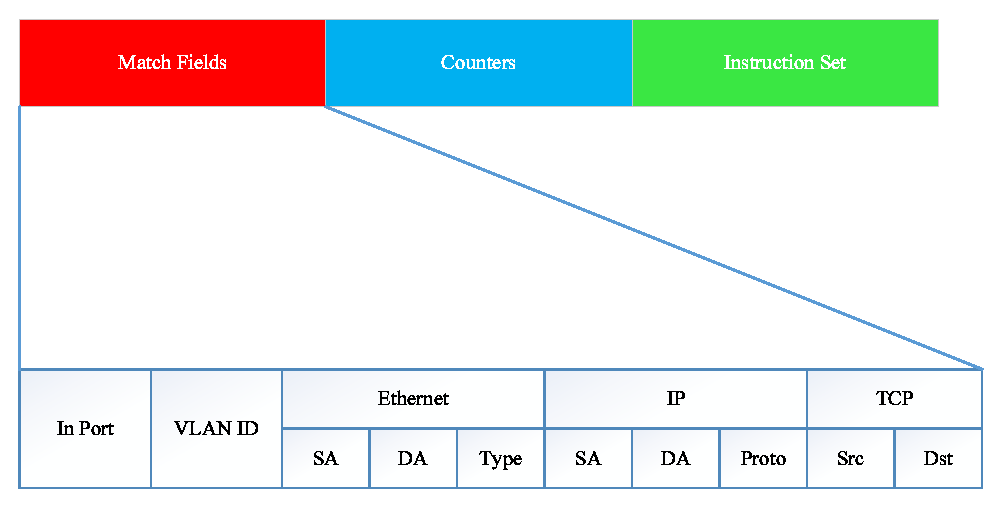
\includegraphics[scale=0.75]{chap2/flowtable.eps}
  \caption{The flow table of OpenFlow1.0}\label{flowtable}
\end{figure}

Everytime a packet reaches an OpenFlow switch, the header fields will be extracted, and compare will the matching field of the flow entries. The comparision starts from the first entry and continues in sequence. When a matching entry is found, the packet will be processed according to the corresponding schemes in that entry. Meanwhile, the value of counters will be modified when there is a match. If no matching entries are found, the switch will take actions refering to the table-missing records in the flow table. Each flow table must have a table miss record, in order to deal with situations where no match is found. In this record, a set of instructions will be defined, such as discarding the packet, flooding the packet, or forwarding the packet to the controller. The process is shown in Figure \ref{switchact}.

\begin{figure}[htbp]
  \centering
  % Requires \usepackage{graphicx}
  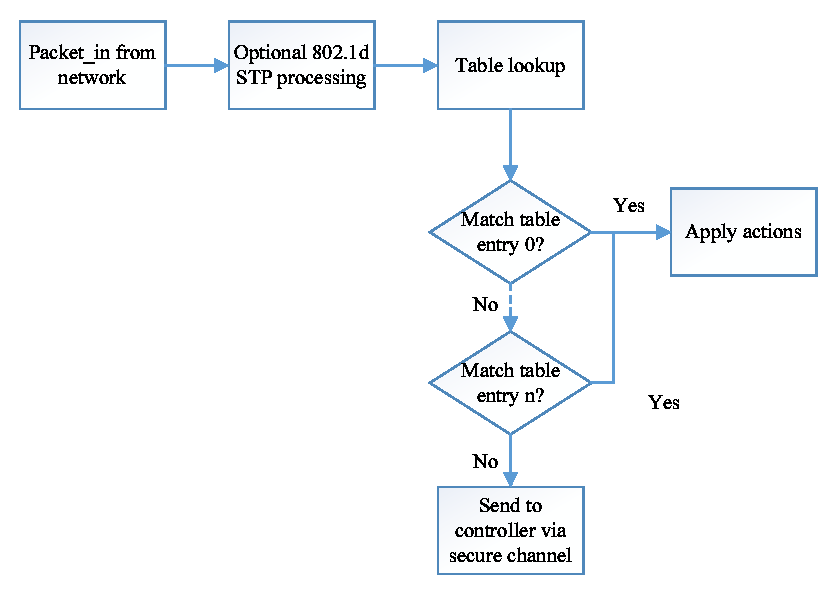
\includegraphics[scale=1]{chap2/switchact.eps}
  \caption{Packet Flow in an OpenFlow Switch}\label{switchact}
\end{figure}

\subsection{The Structure of OpenFlow}
\label{sec:The Structure of OpenFlow}

OpenFlow is the core of SDN ,and basically has the similar structure as SDN. In OpenFlow framework, the most important two parts are the OpenFlow controllers and the OpenFlow switches. Every switch in the network has to connect to at least one controller, and communicates with the controller using standard API. Then the controller runs an application that control and manage the network. Everytime a decision is needed, the OpenFlow switch has to request the OpenFlow controller. For example, if a new packet is send to a switch, the switch will ask the controller how to manage this packet\_in event. Then the controller has to make decisions according to its inside strategies, and tell the switch to forward the packet or just discard it. The structure of OpenFlow can be seen in Figure \ref{opstructure}.

The OpenFlow switch consists of a secure channel and a flow table. After OpenFlow 1.3, the table is changed to a multi-level flow table that has 256 levels. The secure channel is a module that is used for switches to communicate with the controller, and the connnection between switch and controller is realized by sockets. And the flow table is used to save the routing rule of data packets. When data packets come into a switch, it will find the matching rule in the flow table and take corresponding actions. Otherwise, a packet\_in message is generated.

\begin{figure}[htbp]
  \centering
  % Requires \usepackage{graphicx}
  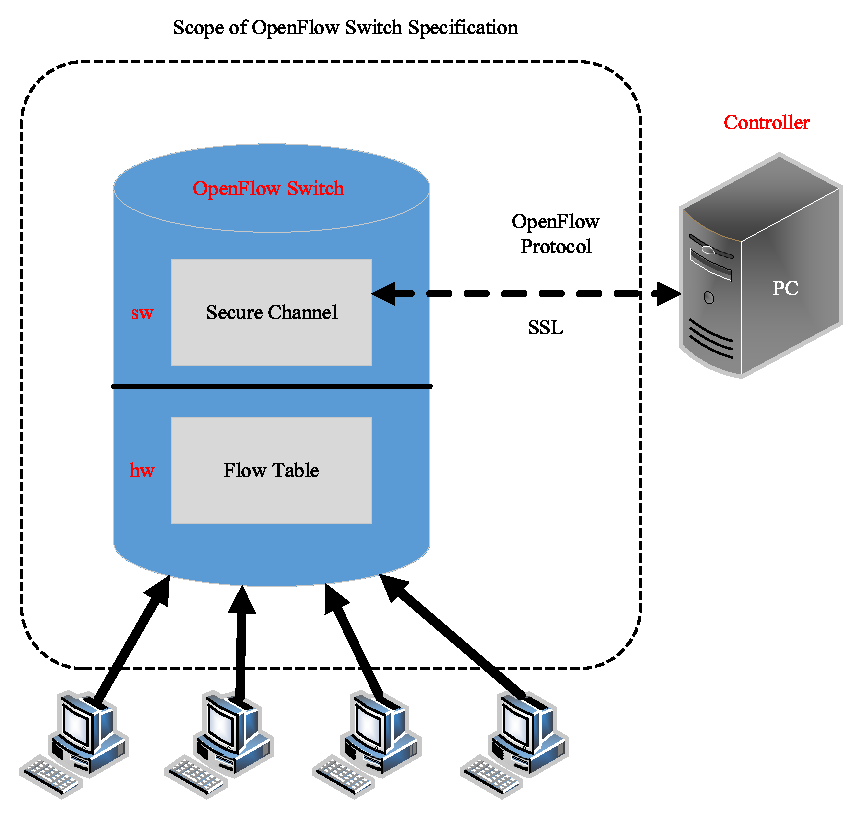
\includegraphics[scale=0.75]{chap2/opstructure.eps}
  \caption{The basic structure of OpenFlow}\label{opstructure}
\end{figure}

Compared to traditional switches, the switches of OpenFlow have a matching level of four, but the traditional switches only have a layer of two. Meanwhile, we can run OpenFlow protocols on OpenFlow switches, and thus implement many functions of a router. Currently, OpenFlow switches can be obtained in three ways: physical OpenFlow switches, installing Open VSwitch (OVS) on physical computers, or using the mininet simulation environments. In this paper, we will use mininet to set up an OpenFlow network and test our algorithms.

There are also many types of OpenFlow controllers, such as pox, ryu, OpenDayLight, etc., which we will compare and discuss later. The controller is mainly divided into three parts in the function level: the communication module in the bottom layer, upper layer applications and the OpenFlow protocols. Since the controller and the switches are linked by sockets, the bottom layer of communication module is also implemented as a socket. And the upper layer applications can be customly developed by users, such as an l2 learning switch.

Another important concept in OpenFlow structure is its port. The port of OpenFlow is a kind of interface with which OpenFlow passes data packets between its controlling process and the rest part of the network. Logically, each pair of switch are connected using an OpenFlow port. The set of OpenFlow port may not be exactly the same as the network port provided by the hardware switch, since some Internet port of the hardware may be disabled by OpenFlow, and OpenFlow may also define extra ports that developers want to use. 

An OpenFlow switch must support three kinds of OpenFlow ports: the physical port, the logical port and the reserved port. The physical ports of OpenFlow are ports defined by switches, corresponding to the hardware ports of a switch. In some kinds of deployments, OpenFlow switches can achieve hardware virtualization of switches. In these conditions, the physical switches of OpenFlow can represent a virtual slice that corresponds to the hardware port of a switch. The logical port of OpenFlow is also defined by switches, but there is not a direct mapping between the logical port and a certain hardware port. It is a higher abstract concept, and may be the ports that do not use OpenFlow in the switches. Meanwhile, the logical ports can be mapped to different physical ports, and the processing of logical ports must be transparent to OpenFlow. The only difference between physical ports and logical ports is that: a data packet sending to a logical port may contain an extra metadata field -- the tunnel ID. And when a message received on the logical port is being sent to the controller, both its logical ports and the physical ports will be acquired by the controller. The reserved port of OpenFlow is used for certain forwarding actions, such as sending to controllers, flooding, or forwarding using methods except OpenFlow, as the traditional switches do.

From the overall point of view, the idea of OpenFlow is in fact quite clear. The network devices maintains a flow table and forward packets according to this flow table. Meanwhile, the generation, maintainment and distribution of this flow table are all implemented by an outside controller. This structure that separates the control plane and data plane means that, for L2 switches, the learning of MAC address will be realized by controller, and the basic L3 routing configurations will also be distributed to switches by this controller. For L3 devices, the Interior gateway protocols (IGP) and the Exterior gateway protocols (EGP) both run on the controller, and are distributed to corresponding routes according to different requirements. The distribution of flow tables can be active as well as passive. In the active pattern, the controller will send the collected information of flow table to network devices once in a while, and later the devices can forward data packets according to the flow table. In the passive pattern, when the network devices receive a message that does not have a match in the flow table, it will send the message to the controller, and let the controller to decide how to forward this message. Then the controller will also distributed related flow tables to the switches.

\section{Principles of Load Balance}
\label{sec:Principles of Load Balance}

Load Balance is a technology that allocates the load to two or more computers, CPU, or other kind of resources adequately in parallel computing, so that we can optimize the resource allocation, maximize the throughput of the processors, and minimize the respond time.

\subsection{Classification of Load Balance}
\label{sec:Classification of Load Balance}

Load Balance is usually classified to several types according to different use cases. In the situation of local traffic management, we usually assort it into two types: static and dynamic. And in the mode of cluster service, we usually divide it to persistent load balance and non-persistent load balance. 

The performance of a cluster is usually directly decided by the design of the balancing schemes. In general, the main duty of the load balance algorithm is to decide how to choose a node in the cluster, and send new coming requests to it, or migrate the jobs to it from other overloaded nodes. There is no omnipotent schems that suits all situations. Thus when we have to design a load balancing strategy, we have to take the features of the cluster, and combine different technologies and algorithms. The basic algorithms used in load balance are listed below:

\textbf{Round Robin} : The Round Robin method is the easiest one to implement in all scheduling algorithms. In a task queue, all the members have the same importance, and the algorithm will choose the next node in sequence. The actions of this algorithm can be predicted, and each node has a possibility of 1/N to be chosen. Thus it is easy to calculate the load distribution in this condition. The Round Robin method is usually used in situations where all the nodes have similar abilities.

\textbf{HASH} : By using an injective and irreversible HASH function, the HASH method send the Internet request to the certain node calculated by the function. The HASH method shows its ability when other load balance algorithms are not very useful, for example, in UDP sessions. 

\textbf{Least Connection Method} : In the Least Connection method, the load balancer records all active connnections, and send the new request to the node that has the least connection at the current time. This method is usually used for problems corresponding to TCP links.

\textbf{Minimum Connection Method} : In Minimum Connection method, the load balancer records the requesting conditions of all nodes during a period of time, and send the next request to the node that has the least total connections during this time. It keeps the number of total connections instead of the current connections, compared to Least Connection Method.

\textbf{Fastest Responding Method} : The load balancer keeps the responding time from itself to each nodes in the cluster, and sends the request to the nodes with the fastest responding speed. In most of the clusters that based on LAN, this method does not perform very well, since the ICMP package can basically respond in 10ms. This means that the difference among different nodes can not be shown very clearly. However, if this method is used on WAN, then it will perform quite well, especially in the topologies that are divergent.

\textbf{Weight Method} : This method can only be used together with other methods. By allocating different values (priorities) to different nodes, it establishes a priority queue. In this queue, nodes with the same priority can be dealed with the Round Robin method or Least Connection method. Here, the priority should be an estimated value based on the ability of each node.

\subsection{Challenges of Load Balance}
\label{sec:Challenges of Load Balance}

Currently portal websites and search engines are becoming more and more popular among people, thus leading to a huge amount of page view every second. This will cause great pressure on the devices of data center networks. Thus, needless to say, devices of load balance are attracting attention from various areas. Nowadays, the load balancers are usually divided into two types: hardware devices, and software load balancers such as Linux Virtual Servers. And most of the network are using both of them. However, we can still discover there are a lot of challenges in this area:

\begin{enumerate}
\item \textbf{The pre-defined trend of load balancer}\\
Since the performance of load balancer may vary a lot in different situations, current load balancers are usually pre-defined for certain applications or certain products. Thus, this condition makes it hard for users to reuse the codes. And users will also meet a lot of trouble if they want to compare different load balancing strategies on these load balancers. Since they are pre-defined, they usually have a strong dependency on a certain kind of structures, preventing users from transplanting it to other platforms.
\item \textbf{The collaboration among multiple load balancers}\\
As the scale of the network increases, a single load balancer cannot satisfy the frequent requests sent by hosts. Thus, the administrator of the network may want to use multiple load balancers to monitor the network. In this way, the processing logic inside each load balancer shall be designed very carefully, considering the potential problem of information sharing, synchronization and control migration.
\item \textbf{The complex hardware and software system}\\
Though we can develop our own software defined load balancers, it will still run on hardwares. Thus, the deployers have to consider the cost of maintaining network devices, or replacing old devices with newer ones. Meanwhile, if the structure of the SDN is changed, there will also be a cost on this update. Of course, the periodical test and update of the algorithm of this load balancer should also be considered.
\end{enumerate}

Refering to the structure of SDN and OpenFlow, we may find that similar problems will occur if we deploy load balance algorithms in it. Thus, there are still a lot to do in this area.

\section{OpenFlow Protocols}
\label{sec:OpenFlow Protocols}

The communication between a switch and a controller is realized using OpenFlow Protocols specified by Open Networking Foundation (ONF) \cite{onf}, by sending a predifined message between them through the secure channel. The secure channel is an port that connects each switch to its controller. When the switch starts, it will start a Transport Layer Security (TLS) connection with the controller defined by users. The switches and controllers will check the status of each other using a certificate. The OpenFlow protocols can be regarded as a possible implemention of switch-controller interactions (the southern interface), since it defines the communication between switch hardware and network controllers. However, some fine grained security choices are still not concerned in current standards.

OpenFlow protocols defined three kinds of message types, each can be further devided into several subtypes: controller-to-switch, symmetric, asynchronous. 

\subsection{Controller-to-switch Messages}
\label{sec:Controller-to-switch Messages}

The controller-to-switch message is started by the switch, and is used for directly managing the switches or check the status of switches. This kind of message may or may not require a response and can be divided to the following subtypes:

\textbf{Features} : When establshing a TLS session, the controller will send a feature request to the switch, and the switch must answer the request using a feature message. The message will include the functions that the switch supports in detail.

\textbf{Configuration} : Controllers can set and query the configuration parameters in the switch, and the switch will only respond to the query message.

\textbf{Modify-State}: This message is sent by controller, and is used for managing the state of switches. We can use this message to add, modify or delete the flow entries in the flow table, or set the priority of switch ports. 

\textbf{Read-State} : This kind of message collects statistics from the flow table, ports or flow entries from the switch.

\textbf{Packet-Out} : Controllers use this message to send packets from a designated port of switch.

\textbf{Barrier}: Controllers use a Barrier request and the response to make sure the dependency of information, or receive the notification that the actions are completed. We will use this message for synchronization purpose in our scheme.

\subsection{Symmetric Messages}
\label{sec:Symmetric Messages}

Symmetric messages can be sent from a controller to a switch, and can also be sent from a switch to a controller. There are usually three types of symmetric messages:

\textbf{Hello} : The Hello message is used for controllers and switches to establish a connection. After the connection is set up, they will send each other a Hello message to make sure the success.

\textbf{Echo} : Both controllers and switches can send an Echo message to the other side. The receiver must reply the message. This message is used for testing delays and check whether the connection is still kept. In other words, it can be used for 'heartbeat' messages.

\textbf{Vender} : The Vender message is always kept for future versions. It makes use of the OpenFlow space and intends to offer a standard way to extend the function of OpenFlow.

\subsection{Asynchronous Messages}
\label{sec:Asynchronous Messages}

The asynchronous messages are started by the switches, and is used for notifying controllers the network events and the changes of switches' status. A switch sends the asynchronous message to the controller when a data packet arrives, the status of the switch changes, or an error occurs. Four types of Asynchronous messages are usually seen:

\textbf{Packet-in} : When switches receives a packet, it will try to find a match in its flow table, and then follow the actions defined in that flow entry. However, if no matches are found, or if the packet is required to be sent to the controller, the switch will then send a packet-in message to the controller. For switches that have enough space to store this packet, it will include the part of the header field and the buffer ID in the packet-in message. Otherwise, the switch must include all the data of that packet in this packet-in message.

\textbf{Flow-removed} : As we have said before, there is a limited space for flow tables to store the flow entries. Thus when the flow table is full and a new entry is to be added, the counters will find the most inactive flow entry and delete that. And in fact, each flow entry have a life period, the switch will delete that entry if it exceeds its living time. In these two conditions, the switch will generate a flow-removed message.

\textbf{Port-status} : When the configuration status of a switch changes, it will send a port-status message to the controller.

\textbf{Error} : This message is used to notify the controller that there is an error.

\subsection{Communication Process}
\label{sec:Communication Process}

When an OpenFlow connection is established, both the controllers and the switches have to send an OFPT\_HELLO message to the other side. This message will include the highest version number of supported OpenFlow protocols in each side. The receiver will use the lowest protocol version that is supported by both side. As soon as a sharing version number is found, the connection will be established successfully. Else an OFPT\_ERROR message will be sent and breaks the link.

When an error occurs, the switch will attempt to connect to the backup controller. If all the attemptions fail in the end, the switch will come into the emergency model, and reset all the TCP links. Only flow entries of the emergency model will be matched during this time, and all other entries will be deleted.

\subsection{Role of controllers in a multiple controller situation}
\label{sec:Role of controllers in a multiple controller situation}

Multiple controllers are supported in OpenFlow 1.3 \cite{opproto}. However, this multiple controller situation is only meaningful for the switches. Since OpenFlow is a protocol used for communication between controllers and switches. The communication between controllers and how the controllers cooperate is not concerned in OpenFlow.

Compared with the switches, the controllers have three types of roles in OpenFlow 1.3: equal, master and slave. A controller can change its role at any time.

\textbf{OFPCR\_ROLE\_EQUAL} : This means the controller is an equal controller. It has all of the permissions, and has the same role as other equal controlles. For example, if a switch connects to three controllers, and the role of all these controllers are equal. Then any one of the controllers has the same importance for the switch.
\textbf{OFPCR\_ROLE\_SLAVE} : This means the controller has the role as a slave. It has read-only permissions, and does not receive asychronous messages except for port\_status message. Meanwhile, this controller cannot send following messages (messages for writing purpose): packet\_out, flow\_mod, group\_mod, port\_mod, table\_mod\_request and table\_features. An error message must be replied if a switch receives above messages from a slave controller. There can be many slave controllers in the network.

\textbf{OFPCR\_ROLE\_MASTER} : This means the controller is a master controller. It has the same permission as an equal controller. The only difference is that, there can only be one master controller in the system, but can have many equal controllers.

\subsection{Evolvement of OpenFlow Versions}
\label{sec:Evolvement of OpenFlow Versions}

Since OpenFlow 1.0 has been released in 2009, this protocol has experienced an obvious evolvement in its following versions 1.1, 1.2, 1.3 and 1.4. The currently most popular version is OpenFlow 1.0, and OpenFlow 1.3 is also accepted by more and more companies. Figure \ref{evolvement} shows the difference between these two versions.

\begin{figure}[htbp]
  \centering
  % Requires \usepackage{graphicx}
  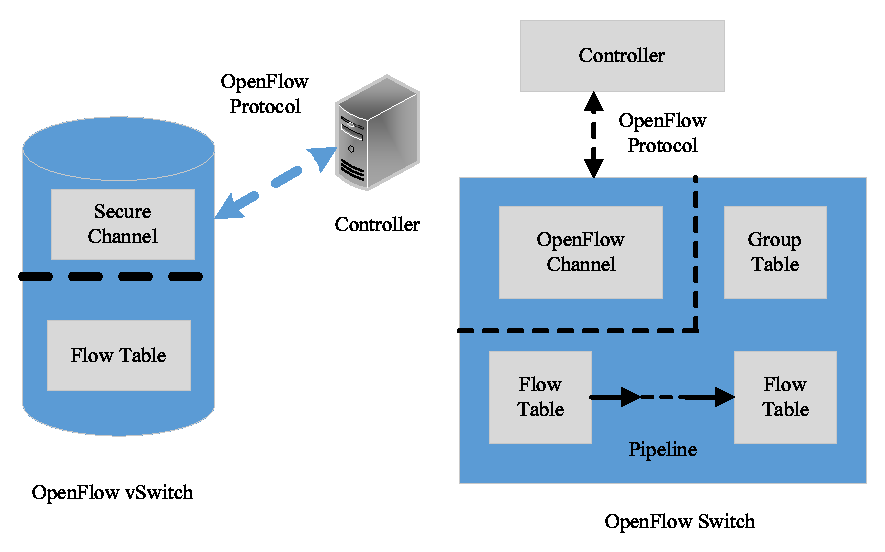
\includegraphics[scale=1]{chap2/evolvement.eps}
  \caption{The difference between OpenFlow version 1.0 and 1.3}\label{evolvement}
\end{figure}

Let us have a short review of the evolvement history of OpenFlow, which is quite important if we want to make a research on multiple controllers in OpenFlow network.

In OpenFlow 1.0, there is a flow table in every OpenFlow switch, which is used for searching, processing and forwarding the packets. Each switch is only allowed to communicate with one controller, and the maintainment of the flow table is also realized by corresponding OpenFlow messages sent by the controller. The advantage of this version is that it is totally compatible with current commmercial chips. Companies can deploy OpenFlow 1.0 in their traditional switches, just by updating the firmware. Thus, OpenFlow 1.0 is the most popular version nowadays.

From the version of OpenFlow 1.1, this protocol begins to support multi-level flow tables. By dividing the flow table matching process into several steps and make it working in a streamline, we can avoid the problem that a single flow table is over-expanded with so much information. Meanwhile, the concept of Group is also used in OpenFlow 1.1, making it possible to perform the same actions by citing the same group tables in different flow entries.

Then in OpenFlow 1.2, users are allowed to define their own matching fields, under the definition of OpenFlow Extensible Match (OXM). Meanwhile, in this version, a switch is allowed to connect with several controllers, and the controllers are allowed to change their role by sending ROLE\_REQUEST messages.

In April, 2012, another long-term support version OpenFlow 1.3 is released. In this version, more matching keywords are allowed. And it permits controllers and switches to decide the protocol versions to be used, by negotiating in the start phase of the connection. One year later, OpenFlow 1.4 was released, and made several improvements in the control plane, but was still based on OpenFlow 1.3.

\section{Controllers used in OpenFlow network}
\label{sec:Controllers used in OpenFlow network}

Several kinds of controllers are widely used at the moment. Among them, POX, OpenDayLight, Floodlight, Beacon and Ryu are the most popular ones. In this experiment, we will use Ryu controller to monitor the whole network. Other controllers will be introduced and compared later.

\subsection{Introduction to Ryu}
\label{sec:Introduction to Ryu}

Ryu \cite{ryu} is a SDN controller developed by Nippon Telegraph \& Telephone (NTT) in Japan.
This controller is implemented by Python, and users can realize their own applications using Python. Ryu has support for several versions of OpenFlow at the moment, including OpenFlow 1.0, OpenFlow 1.2 and OpenFlow 1.3, It also has support for deploying applications on OpenStack. The application programming model of Ryu is shown in Figure \ref{ryueps}.

\begin{figure}[htbp]
  \centering
  % Requires \usepackage{graphicx}
  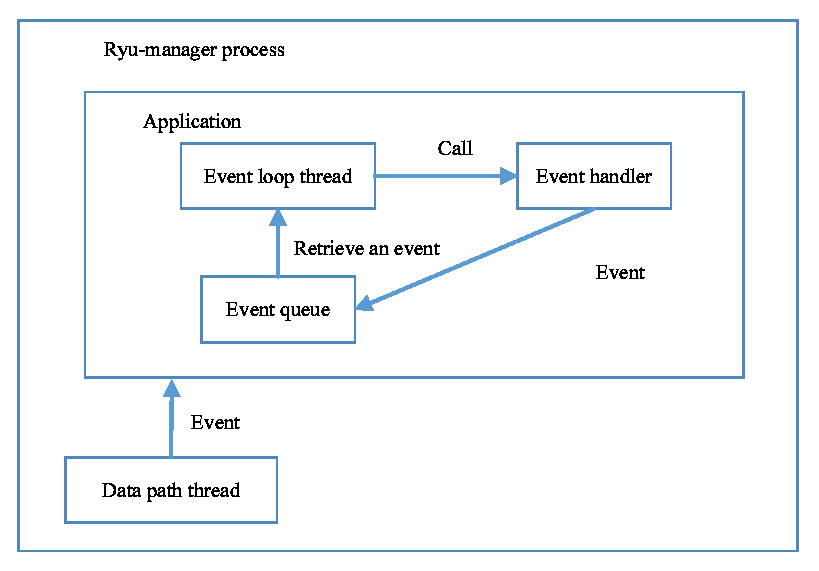
\includegraphics[scale=1]{chap2/ryu.eps}
  \caption{Application programming model of Ryu}\label{ryueps}
\end{figure}

The code of the main controller is organized under the /ryu/ryu/ folder. Let's have a short introduce on the main structure of Ryu code.

\begin{itemize}
\item app/ - Contains several applications that can run directly on the controller
\item base/ - Contains the basic classes of applications. The most important document in this folder is app\_manager.py. This document is the central manager of an Ryu application, which is used for loading the application, receiving messages and finishing the routing. The RyuApp class is defind in this file.
\item controller/ - Contains several important files to handle OpenFlow functions, such as events.py, ofp\_handler.py, controller.py, etc. The basic class OpenFlowController is defined in controller.py, which is used to define an OpenFlow controller and dealing with connections between controllers and switches.
\item lib/ - Defines the basic data structures, such as dpid, mac and ip.
\item ofproto/ - Contains two types of files: the definition of the data structure of OpenFlow protocols, and the related parsers for these protocols. 
\item topology/ - Contains codes for discovering the topology of OpenFlow network.
\end{itemize}

Then we used the hub application as an example to elucidate how to write a controller application in Ryu. The code is as follows:

\begin{lstlisting}[language={python}, caption={hub.py written by Ryu}]
from ryu.base import app_manager
from ryu.controller import ofp_event
from ryu.controller.handler import MAIN_DISPATCHER
from ryu.controller.handler import set_ev_cls

class L2Switch(app_manager.RyuApp):
    def __init__(self, *args, **kwargs):
        super(L2Switch, self).__init__(*args, **kwargs)

    @set_ev_cls(ofp_event.EventOFPPacketIn, MAIN_DISPATCHER)
    def packet_in_handler(self, ev):
        msg = ev.msg
        datapath = msg.datapath
        ofp = datapath.ofproto
        ofp_parser = datapath.ofproto_parser

        actions = [ofp_parser.OFPActionOutput(ofp.OFPP_FLOOD)]
        out = ofp_parser.OFPPacketOut(
            datapath=datapath, buffer_id=msg.buffer_id, in_port=msg.in_port,
            actions=actions)
        datapath.send_msg(out)
\end{lstlisting}

In this code, we import ofp\_event at first. ofp\_event is used to define an event, so that we can register a handler in the function and monitor the events as well as reply to them. The main function in this file -- packet\_in\_handler is used to deal with packet\_in events. And we use the signal @set\_ev\_cls to tell Ryu that, when the controller receives a packet\_in event, it will resort to packet\_in\_handler. MAIN\_DISPATCHER represents a general status. The first parameter of set\_ev\_cls represents the function to be used when event happens, and the second parameter tells the switch that, the function can only be called after the connection succeeds.

Then in the function of packet\_in\_handler, ev represents for an event, and ev.msg is a member of ev, which is used to carry the packet that triggers the event. The msg parameter is in fact a packet\_in message, and msg.datapath is used to get the datapath structure of msg, which is used to describe a network bridge. datapath.ofproto is an object of OpenFlow protocol structure, and contains the data structure used later. datapath.ofp\_parser is a data structure used to parse that object. And actions is a list, which stores the actions to be done in the future. The parameter out in this code is a packet\_out structure, containing the necessary informations of how to deal with the packet, and the function datapath.send\_msg() will send the data to the designated datapath.

\subsection{Other popular controllers}
\label{sec:Other popular controllers}

\textbf{POX} : The first OpenFlow controller is NOX written by C++,and POX is a Python-version NOX that only supports developing using Python. We can thus regard POX as a general, open-source OpenFlow controller written by Python. It is also a platform on which users can develop Internet applications and establish their own topologies. The main application area for POX is the researching area. Since most of the researches will not last for a long time, thus POX devotes to provide users with adequate interfaces instead of stable interfaces.

\textbf{Beacon} : Beacon is a fast, cross-platform and modularized controller based on Java. This controller not only supports event-driven actions, but also supports actions that are based on threads. The controller, whose developing process began in 2010, is not used in some researching projects and platforms for experiments. Since Beacon is written by Java, it is capable of running on several platforms such as Linux and Android. Another advantage of Beacon is that, we can start, stop, install or refresh the modules of Beacon even if it is running, and these actions will not influence other unrelated modules.

\textbf{Floodlight} : Floodlight Open SDN Controller is another kind of OpenFlow controller that is written by Java, usually used in enterprise-level applications. Floodlight runs in Java Virtual Machines (JVM), so it may be a little slower than other controller written in C++ or Python. Floodlight is not only a controller, but also a set of applications running on Floodlight controller. Thus Floodlight is usually considered to be composed of three parts: the Floodlight controller, the application compiled with the controller as a Java module, and the network applications over the REST API of Floodlight.

\textbf{OpenDayLight} : OpenDayLight (ODL) controller is a modularized, multi-protocol controller infrastructure that has a high scalability in both scales and functions. It is developed by Java, and can run on any hardware platform that supports Java JVM 1.7 or higher, in the form of a Java virtual machine. OpenDayLight controller not only supports OpenFlow protocols, but also supports other open-source protocols. Meanwhile, it allows communication with other devices with OpenFlow or other protocol agents. Its northern API also supports the collaboration of user defined applications and the controller itself in controlling the network.

%%==================================================
%% chapter03.tex for SJTU Bachelor Thesis
%% version: 0.5.2
%% Encoding: UTF-8
%%==================================================

% \bibliographystyle{sjtu2} %[此处用于每章都生产参考文献]

\chapter{Problem Statement}
\label{chap:problem}

As we have said before, traffic in DCN can be represented as communication between pairs of virtual machines. And in this process, several switches need to be used for them to connect with each other. Since our network is based on the framework of OpenFlow, there are mainly two important components in the system -- controller and switch. The controller will monitor the whole system, and may get global or local information according to its type. For centralized controllers, they can get all information of the network, but for distributed controllers, they will just get information in its neighborhood. When the traffic in the network changes, the controller will distribute routing messages to the flowtable of the switches, according to its built-in strategies. And for switches, each switch may be used by several hosts. There are mainly three kinds of switches -- Top of Rack (ToR) switch, Aggregation switch and Core switch. They are all used for communication in data centers. Inside each switch there is a flowtable. When receiving flows, the switch will refer to its flowtable, and then decide where and how to forward these flows. The flowtable can be added, deleted or modified by controllers. Meanwhile, each entry in the flowtable have its life time. When the time is expired, the entry will be automatically deleted by the switch, in order to give spaces to new schemes. This paper is mainly about load balancing in a DCN, so we omit the details of the routing process.

Then we will define our problem in a formal way. We want to discuss the problem of traffic load balancing with multiple controllers and switches under the framework of Openflow. Each switch can be monitored by several controllers, but only one of these controllers is the master controller. And each controller can also manage several switches. In our DCN that is based on the structure of OpenFlow, we denote the $j$th switch as $s_j$. Since each switch is responsible for several hosts, and the hosts will produce traffic in their communication process, the switch will finally manipulate a certain amount of traffic. We treat this traffic as the weight of the switch, and we use $w(s_j)$ to represent the weight of switch $s_j$. And we use $c_i$ to represent the $i$th controller in the network. Suppose there are $m$ controllers and $n$ switches in the network. The controllers are in the set $C=\{c_1,\cdots,c_m\}$. The switches are in the set $S=\{s_1,\cdots,s_n\}$, and each of the switch has a weight of $w(s_j)$.  Then we would like to make a weighted $m\mbox{-}partition$ for all the switches, such that each controller will take control of a part of the switches, and make the system as balanced as possible. Though a switch $s_j$ can be connected with several controllers, only one of them is the master controller, which can actually manage the switch. Thus, we denote the actual controller (master controller) of as $AC(s_j)$. For all  controllers that switch $s_j$ can be connected with, we call them reachable controller of $s_j$, and use a set $RC(s_j)$ to denote them. In other words, every controller in the set $RC(s_j)$ have the potential to be the actual controller of $s_j$, but only one of them can really be the actual controller in the end. Similarly, for controller $c_i$, it can monitor a set of switches that are within the controlling range of $c_i$, we call this set the reachable switches of $c_i$, and denote it with $RS(c_i)$. And the actual subset of switches that are monitored by $c_i$ is called the actual switch set, and is denoted by $AS(c_i)$. The weight of controller $c_i$ is defined by the total weight of its switches in the actual switch set $AS(c_i)$, and is denoted by $w(c_i)$. Here note that $AC(s_j) \in RC(s_j)$, and $AS(c_i) \subseteq RS(c_i)$.

The symbols used in this paper are listed in Table \ref{table_symbol}: 

\begin{table}[htbp]
\centering
\caption{Definition of Terms} \label{table_symbol}
\vspace{1mm}
\begin{tabular}{l|l}
\hline
%Term&Definition\\
Term & \multicolumn{1}{c}{Definition}\\
\hline
$S, s_j$& the whole switch set that consists of n switches: $S$=\{$s_1,\cdots,s_n$\}\\
$w(s_j)$& the weight of $s_i$, defined as the number of out-going flows.\\
$RC(s_j)$& the reachable controllers set of the $j$th switch.\\
$AC(s_j)$& the actual controller of the $j$th switch.\\
\hline
$C, c_i$& the whole controller set that consists of $m$ controllers: $C$=\{$c_1,\cdots,c_m$\}\\
$w(c_i)$& the weight of $i$th controller, the sum of $AS(c_i)$'s weight. \\
$RS(c_i)$ & the reachable switches set of the $i$th controller.\\
$AS(c_i)$& the actual switches set of the $i$th controller.\\
$AN(c_i)$& the adjacent nodes (logically connected) of $i$th controller.\\
\hline
\end{tabular}
\end{table}

In order to avoid hot controllers in the network, which affects the performance of the whole system, each controller should finally have the same amount of weight, which means that they each process a similar workload. Otherwise, the hot node in the network will slow down the speed of data forwarding. People used to use a centralized controller to deal with this problem, leading to a bottleneck in the network. In our problem definition, we discuss the situation where multiple controllers and switches are used. To make it easier for us to quantify the effect of load balancing in the system, we define the \emph{Standard Deviation} of this multi-controller system as a reference index, denoted by $\sigma=\sqrt{\frac{1}{m}\sum_{i=1}^{m}(w(c_i)-\overline{w(c)})^2}$, in which $\overline{w(c)}$ is the average weight of all controllers. If the traffic flow changes as time passes , the weight of controller $c_i$ may increase or decrease very fast, making it unbalanced comparing to other controllers, and this will lead to the increasement of $\sigma$. Thus in this condition, we have to move some of the switches of the overload controller $c_i$ to other controllers in controller set $AN(c_i)$ which are not that busy.

Then we can firstly define our naive version of this problem as balancing the traffic among $m$ controllers in real time environment. When the balance is broken, we will move switches among all related controllers according to our migration schemes. We define this problem as \emph{Load Balancing problem of Multiple Controllers} (LBMC). In our strategy, the controllers will recalculate mapping between controllers and switches once in a while, and then migrate some of the switches to more appropriate controllers to make the system balanced. The effective area of the controllers may overlap, and each controller will manage to get almost equal load in the end. Figure~\ref{before} and Figure~\ref{after} shows the migrating process and the final state after the migration.
\begin{figure}[htbp]
  \centering
  % Requires \usepackage{graphicx}
  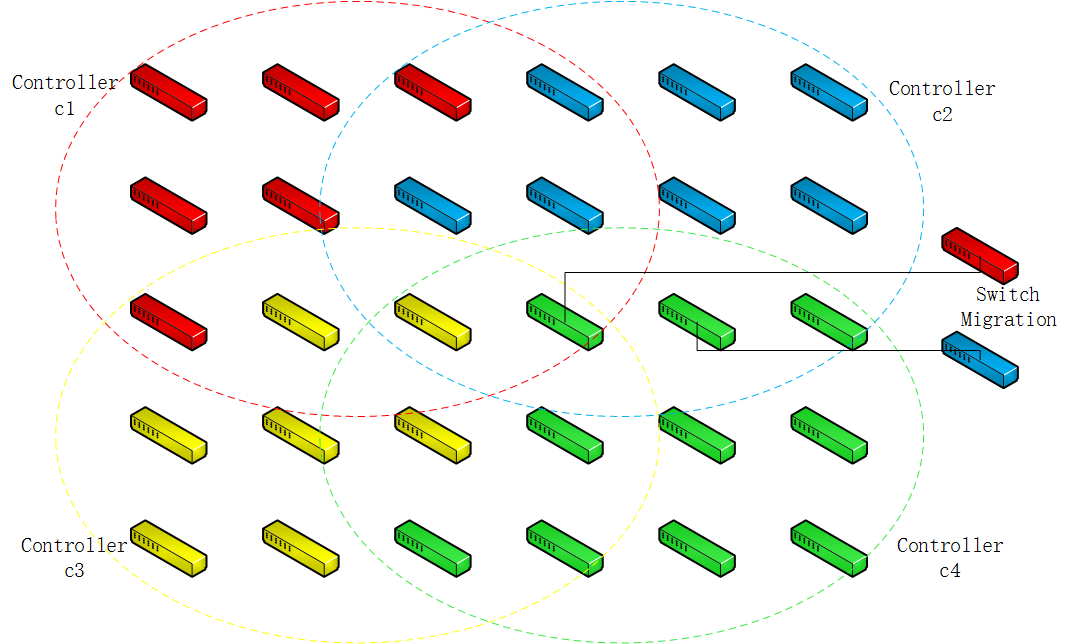
\includegraphics[scale=0.45]{chap3/before_change.png}
  \caption{An example of migrating process. There are 4 controllers in the system, Their effective areas are shown using the ellipses. The overloaded controller $c4$ manages to move the controllers to controller $c1$ and $c3$.}\label{before}
\end{figure}
\begin{figure}[htbp]
  \centering
  % Requires \usepackage{graphicx}
  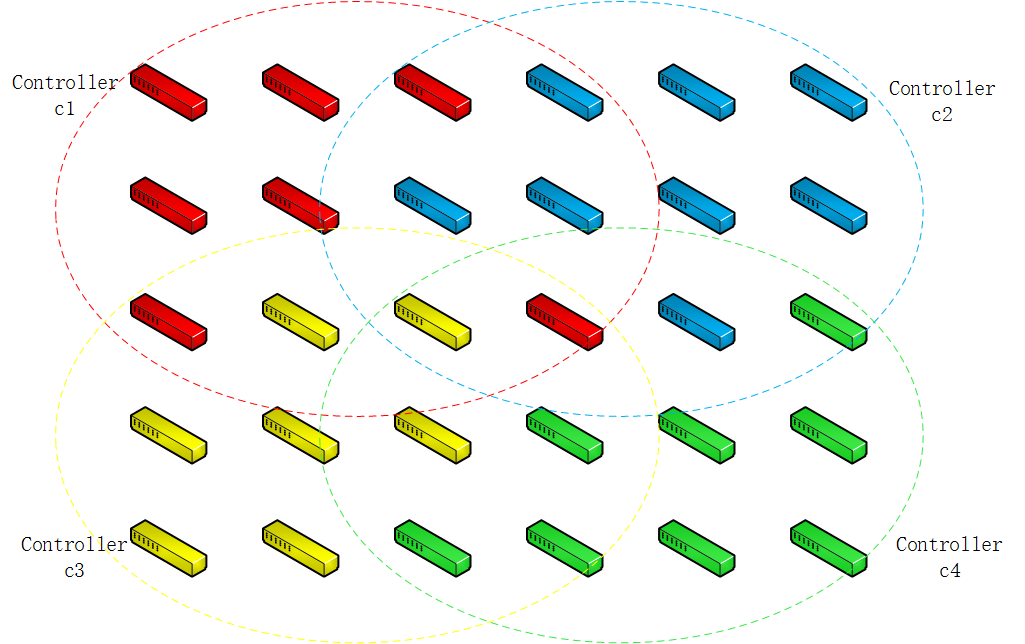
\includegraphics[scale=0.45]{chap3/after_change.png}
  \caption{The final state after the migrating process}\label{after}
\end{figure}

Actually, all the controllers can be illustrated as a connected graph for data communication. If the traffic flows vary a lot, the weight of the controller will also change because of the dynamic weight change of the switch, which leads to the result that the controller is unbalanced with other controllers. Then we must start our regional migration to migrate the switch of this controller to other available controllers to reduce the workload of the controller and keep the entire traffic balance again. The controllers can communicate between each other to ensure all the ToR-to-ToR communication can be handled. Through the above architecture, we can reduce the workload of each controller and routing component efficiently, thus can alleviate the scalability problem and the congestion problem.

We call the above statement ``naive version" because this definition is under an ideal situation. In our problem statement, we omit the performance limit of each controller. That is to say, we suppose that all the controllers in the network are the same, and has an unlimited workload capacity. In fact, in a very large data center, the distributed controllers may have very different features. For example, some of them may have a high capacity, while others have a low capacity. Let us consider the following condition: there are three controllers in the network system, say, $c_1$, $c_2$, $c_3$. The maximum capacity for $c_1$ is $\lambda$, for $c_2$ is 2$\lambda$ and for $c_3$ is 4$\lambda$. The total weight of all switches in this system is 6$\lambda$. If our naive CM-LBMC program works perfectly, then each controller will get the load of 2$\lambda$ in the end. Thus, in this condition, $c_1$ works in an overloaded status, and will definitely become the bottleneck of the system. However, $c_3$ only makes use of 50\% of its maximum abilities.

Meanwhile, we consider all the switches are equal, and all the traffic flows are equal. In Google's B4 network, they come up with the idea of high-priority traffic and low-priority traffic. This is also what we should consider in load balancing problems based on OpenFlow. If the distance between a switch and all its potential controllers are close enough, so that migrating switch $s$ from controller $c_1$ to controller $c_2$ will not influence the processing speed of messages, then we sometimes can just omit the priority of the switches. However, in some distributed data centers that has a very sparse structure, it is better to attach a switch to its nearby controllers. Meanwhile, as we have mentioned, the performance of controllers in the network system may be very different. Some of the controllers may have strong computing capacities, and thus can process messages in a higher speed. In real network systems, sometimes we hope certain messages or certain areas can have a higher priority in the whole structure, and we want to allocate switches in this region to those strong controllers.

Therefore, though for a certain switch $s_i$, it can be attached to any controller $c_j$ of its potential controller set $PC(s_i)$, the performance, or the value of the whole system may vary according to the real mapping strategy. If the value we get for $s_i$ monitored by $c_1$ is $\theta$, and for $s_i$ monitored by $c_2$ is 2$\theta$, then its better to distribute $s_i$ to $c_2$, if the current load of both controllers are below their thresholds.

Thus, in this paper we will later discuss the other two version of LBMC problem, which takes consideration of more realistic situations. But we will first establish the model of naive LBMC problem, the other versions are quite similar to this one.

We define parameter $map_{ij}=\left\{\begin{array}{ll}1 & \mbox{If } c_i \mbox{ monitors } s_j \\ 0 & \mbox{otherwise}\end{array}\right.$, Then the naive LBMC problem can be further formulated as the following linear programming:
\begin{eqnarray}
\min & \sigma=\sqrt{\frac{1}{m}\sum_{i=1}^{m} \left(\sum_{j=1}^n w(s_j)\cdot map_{ij}-\overline{w(c)}\right)^2} & \label{NLP-Object}\\
s.t. & \overline{w(c)}=\frac{1}{m}\sum_{i=1}^m \sum_{j=1}^n w(s_j)\cdot map_{ij} \label{NLP-Avg}\\
     & \sum_{i=1}^m map_{ij}=1, \quad \forall j \in [1, n] \label{NLP-Dominate} \\
     & map_{ij}=0, \quad \mbox{if } s_j \not\in RS(c_i) \mbox{ or } c_i \not\in RC(s_j), \forall i,j \label{NLP-Region}\\
     & map_{ij} \in \{0,1\} \quad \forall i, j \label{NLP-Integer}
\end{eqnarray}
Eqn.(\ref{NLP-Object}) is the standard deviation we said before. Eqn.(\ref{NLP-Avg}) calculates the average weight of all controllers. Eqn.(\ref{NLP-Dominate}) means that each switch can only have one controller as its master controller. Eqn.(\ref{NLP-Region}) means that $map_{ij}$ will be equal to 0 if controllers and switches cannot be connected logically. And Eqn.(\ref{NLP-Integer}) means $map_{ij}$ can only be an integer.

The above integer programming is proved to be NP Complete. And further adaptions to linear programming and its rounding have been discussed by predecessors, and are proved to be theoratically appliable in real conditions. Then in the next chapter, we will discuss our schemes of switch migration, and give our algorithms according to different situations.

%%==================================================
%% chapter03.tex for SJTU Bachelor Thesis
%% version: 0.5.2
%% Encoding: UTF-8
%%==================================================

% \bibliographystyle{sjtu2} %[此处用于每章都生产参考文献]

\chapter{Algorithm Design}
\label{chap:algorithm}

Referring to the linear programming and rounding schemes given by predecessors, we can find a perfect solution to the naive LBMC problem in theoretical level. However, solving such a problem usually wastes a lot of time and thus is quite unrealistic in real time environments. And for this reason, it is very important to design some applicable heuristics for real world systems. So, in this chapter, we come up with both centralized and distributed algorithms for load balancing problems within the OpenFlow framework. We will first give the centralized version of the algorithm, since we believe it is easy to deploy and can achieve better performance. Then we will give the distributed version of the algorithm, which is also practical and effective for real applications.

\vspace{-5pt}
\section{Centralized Migration}
Our scheme of centralized migration is devided into two parts. In the first part, we have to initialize the whole system. That is to say, we will give an initial mapping scheme for controllers and switches. Then after initialization, if the traffic in the network changes and make the system unbalanced, we will come to the second part and use our algorithm to re-balance the system, by moving switches from overload controllers to some idle controllers.

\subsection{Centralized Initialization}
Before the migration part, we need to initialize the whole system. We will allocate switches to one of their reachable controllers by our initialization scheme called CI-LBMC (Centralized Initialization of Load Balancing problem of Multiple Controllers). However, sometimes we will confront the situation where several controllers are logically equal to a certain switch. So we will first give a \emph{Selecting Scheme} to deal with this dilemma.

\emph{Selecting Scheme:} (1) When we have to choose a switch $s_j$ from switch set $S$, we choose the one will the largest weight (the weight represents for the traffic). If several switches have the same weight, we choose the one with the smallest number of reachable controllers, i.e., we choose the one with the smallest $|RC(s_j)|$. If there are still several equal switches, we randomly choose a number, and then choose the switch whose sequence number is nearest to this one. (2) When we have to choose a controller $c_i$ from controller set $C$, we choose the one with the smallest weight. If several controllers have the same weight, we choose the one with the smallest number of actual switches $|AS(c_j)|$. Similarly, we will use a random number to decide if the tie still exists.

The reason why we choose the switch with the smallest reachable controller number $|RS(s_j)|$ is that we have to make each controller carry similar traffic. Choose such switches will fasten our speed of establishing a mapping between controllers and switches. Meanwhile, even though we skip the initialization process, our migration schemes will manage to balance the system. So to save time and space, we only give the initialization scheme of naive centralized LBMC and distributed LBMC. The corresponding initialization algorithm for modified LBMC are similar to this one and are easy to think. So we will omit them here. 

Then we show our algorithm of CI-LBMC as Alg.~\ref{Alg-CI}.
\vspace{-4mm}
\begin{algorithm}
%\SetAlgoNoLine
%\dontprintsemicolon
%\SetNoline
\caption{Centralized Initialization (CI-LBMC)} \label{Alg-CI}
\SetKwInOut{Input}{Input}
\SetKwInOut{Output}{Output}
\Input{$S$ with $w(s_i)$; $C$ with $w(c_i)$;}
\Output{The initial mapping scheme of $C$ and $S$}
\BlankLine 
%Compute $Avg_{last}=\sum w(c_i)/m$\;
$IdleList$=\{$s_1$,$s_2$,$\cdots$,$s_n$\}\;
\lnl{InRes1}\While{$IdleList \neq \emptyset$}{
Pick $s_j$ from $IdleList$\;
\eIf{$|RC(s_j)|=1$}{
Allocate $s_j$ to the only controller $c$ in $RC(s_j)$\;
Set $AC(s_j)$ to be $c$\;
Add $s_j$ to $AS(c)$\;
}
{
Allocate $s_j$ to the $c_i$ that has minimum $w(c_i)$ in $RC(s_j)$ \;
Set $AC(s_j)$ to be $c_i$\;
Add $s_j$ to $AS(c_i)$\;
}
Remove $s_j$ from $IdleList$\;
}
\end{algorithm}
\vspace{-4mm}

The initialization algorithm CI-LBMC is based on the idea of greedy algorithm. We have to search the $IdleList$ to establish the link between a controller and a switch. This process will take $O(n)$ time to run in the worst condition. For each switch chosen in the $IdleList$, the \emph{While} loop will have to be run for once, and this loop will take $O(n)$ time to execute, n is the larger one of the controller number and the switch number. Thus in the worst condition, this algorithm will have a time complexity of $O(n^2)$. And for space complexity, since we need to store the reachable and actual mapping relationship of controllers and switches, it will be better if we use matrices to store those information. Thus, the space complexity is $O(n^2)$.

Thus we finish the initialization part, and for normal networks, this CI-LBMC algorithm should have a very good performance. However, since the traffic of the system changes as time passes, we have to come up with another algorithm to reallocate switches to controllers if the balance of this network breaks. To make it easy, we first start from the condition that controllers are all the same and have unlimited capacity, and all the switches are logically equal to controllers in their reachable controller set. Then we will give our naive migration algorithm, which is called the NCM-LBMC (naive centralized migration of LBMC).

\subsection{Naive Centralized Migration}
When the traffic of the whole network changes, we have to find a reference index to decide when we need to migrate the switches. Here we use a threshold to decide the load status of a controller. If the weight of this controller exceed the threshold, then we regard this controller as overloaded, which means its actual switches may be moved to other less-loaded controllers. On the other hand, if the load of this controller does not exceed its threshold, then its switches will not be moved away. In this condition, it may accept switches in its reachable switch set, from other overloaded controllers. From the research of the predecessors, we can notice that the traffic in a data center network is usually changing in a linear pattern. So we can refer to the definition of threshold in Round-Trip Time(RTT), and consider both the effect of current load and historical thresholds. And three parameters are needed, we denote them as $\alpha$, $\beta$ and $\gamma$. These three parameters are related to the characteristic of this data center network, and we have $0\le\alpha\le1$, $\beta > 1$ and $\gamma > 1$. In this algorithm, We will run NCM-LBMC periodically, and remap the whole system if the balance is broken. We denote the threshold and effluence that we will use in NCM-LBMC as $Thd$ and $Efn$, and use parameter $Thd_{last}$ and $Avg_{now}$ to denote the threshold of the last round and the average load of the current round respectively. $Thd$ and $Efn$ will both be used in the algorithm, for us to decide whether we need a migration and how to execute the migration. During each round, we will collect the information of the current system, and calculate the average load of each controller using $Avg_{now}=\Sigma w(s_j)/n$ or $Avg_{now}=\Sigma w(c_i)/m$.

The threshold $Thd_{now}$ and the effluence $Efn$ can be computed as follows:
\[Thd_{now}=\alpha \cdot Avg_{now} + (1-\alpha) \cdot Thd_{last},~ Efn=\beta \cdot Thd_{now}\]

Our basic idea in NCM-LBMC is the greedy algorithm, i.e., we greedily move the switch with the maximum weight to the controller that has the minimum weight. In Alg.~\ref{Alg-CM}, we will show the naive version of our centralized LBMC migration.

The naive version of CM-LBMC consists of five steps. In Step 1, we search the whole list, and find all controllers that exceed the effluence, then we add it to the OverList, in which we store the controllers that are overloaded, this step will take $O(n)$ time to run. Then in Step 2, the algorithm searches the $OverList$ to find the controller $c_k$ with maximum weight, which takes $O(n)$. Next, we move the switches from overloaded controllers that are in the $OverList$, to comparatively  controllers repeatedly. This step takes $O(n^2)$. To decrease the influence of coincidences, we use Step 3 that execute Step 2 for many times to make the $RepeatList$ stable. This step will take the time complexity of $O(n^3)$ in the worst case. In the following two steps, we start a local migrating process in each connected components, still using the idea of greedy algorithm, these steps will take at most $O(n^3)$ time in the worst case. Thus in NCM-LBMC, the whole time complexity is $O(n^3)$. As mentioned by predecessors, we can reduce the time complexity to $O(n^2)$ if we use a priority heap to store the lists. The space complexity we need is still $O(n^2)$ since it will share the same information as the initialization algorithm.

\vspace{-4mm}
\begin{algorithm}
%\SetAlgoNoLine
%\SetVline
%\dontprintsemicolon
%\SetKwIF{If}{ElseIf}{Else}{if}{then}{else if}{else}{endif}
%\SetAlgoVline
\SetKwInOut{Input}{Input}
\Input{$S$ with $w(s_i)$; $C$ with $w(c_i)$; $OverList=RepeatList=\{\emptyset\}$;}
\BlankLine

\textbf{Step 1:}
%Linear expectation:\\
%$Thd=Avg_{now}\alpha + Avg_{last}(1-\alpha)$\;
%$Efn=\beta \times Thd$\;
If $w(c_i)>Efn$, add $c_i$ to $OverList$ \;
%$PendList=OverList=\{\emptyset\}$\;
\textbf{Step 2:}
Search the $OverList$, and select $c_k$ with maximum weight\;
\eIf{$\exists c_l\in AN(c_k)$ and $w(c_l)<Thd_{now}$}{
\Repeat{$w(c_k)\le Thd_{now}$ or $w(c_s)\ge Thd_{now}$}{
Pick $s_p$ of max weight in $AS(c_k)$, search $RC(s_p)$:\\
\eIf{$\exists c_s \in RC(s_p)$ and $c_s\in AN(c_k)$ and $w(c_s)<Thd_{now}$}{
Migrate $s_p$ to $c_s$\;
Set $AC(s_p)$ to be $c_s$\;
Add $s_p$ to $AS(c_s)$\;
Remove $s_p$ from $AS(c_k)$\;
}
{Ignore the current $s_p$ in $c_k$\;}
}
if still $w(c_k)> Efn$, move $c_k$ to $RepeatList$;
}
{
Move $c_k$ from $OverList$ to $RepeatList$;
}

\textbf{Step 3:}
Repeatly execute Step 2 until $OverList=\{\emptyset\}$\;
Let $OverList=RepeatList$, Repeat Step 2 for several times until $RepeatList$ become comparatively stable\;
\textbf{Step4:}
Now we treat $RepeatList$ as a graph, there are some connected components $CC_i(1\le i\le |CC|)$\;
\For{each $CC_i\in CC$}{
We denote $AN(CC_i)=\bigcup_{c_j\in CC_i}AN(c_j)$;
Compute $Avg_{local}=\frac{w(CC_i)+AN(CC_i)}{|CC_i|+|AN(CC_i)|}$\;
\If{$\exists c_j\in CC_i$: $w(c_j)> \gamma \cdot Avg_{local}$}{
Migrate the $s_{max}\in AS(c_j)$ to $c_{min}\in AN(CC_i) \cup CC_i$ repeatedly until $w(c_j)\le \gamma\cdot Avg_{local}$\;
remove $c_j\in CC_i$ from $RepeatList$\;
}
}
\textbf{Step5:}
Repeat Step 4 until $RepeatList$ become stable. Then stop the algorithm.

\caption{Naive Centralized Migration (NCM-LBMC)}\label{Alg-CM}
\end{algorithm}
\vspace{-4mm}

\subsection{Centralized Migration with Capacity Limits}

In our naive version, we simply suppose that all controllers in this network have unlimited processing abilities. However, in real conditions, the performance of each controller will have its upper bound. So if we just use the naive version, though every controller will have almost the same traffic load after several rounds, some of them will work in an overloaded state. For example, let us consider the following condition: there are three controllers in the network system, say, $c_1$, $c_2$, $c_3$. The maximum capacity for $c_1$ is $\lambda$, for $c_2$ is 2$\lambda$ and for $c_3$ is 4$\lambda$. The total weight of all switches in this system is 6$\lambda$. If our NCM-LBMC program works perfectly, then each controller will get the load of 2$\lambda$ in the end. Thus, in this condition, $c_1$ works in an overloaded status, and will definitely become the bottleneck of the system. However, $c_3$ only makes use of 50\% of its maximum abilities. So in fact, the naive CM-LBMC algorithm only balances the value of load among devolved controllers, instead of balancing the performance of processing traffic load.

Therefore, we have to consider the performance limit of each controller when we design a new centralized algorithm. We call this algorithm limited centralized migration of LBMC (LCM-LBMC). To reconfigure the system when it is unbalanced, we still need a threshold parameter and an effluence parameter for each controller. Since different controllers will have different value of these two parameters, we use two sets to store them, $ThdList$ = \{$Thd_1$,$\cdots$, $Thd_n$\} and $EfnList$ = \{$Efn_1$, $\cdots$, $Efn_n$\}. For a certain controller $c_i$, we use ${Des_{now}}^{i}$ to denote its deserved workload of the current sample round, and use ${Des_{last}}^{i}$ to denote the deserved workload of the last sample round. The threshold $Thd_i$ and effluence $Efn_i$ of controller $c_i$ is still computed as follows:
\[Thd_i=\alpha{Des_{now}}^{i} + (1-\alpha){Des_{last}}^{i},~ Efn_i=\beta \times Thd_i\]

The maximum load that controller $c_i$ can hold is denoted as $w_m(c_i)$, and we use $\epsilon$ to denote the percentage of resources to be used for each controller. And another thing to mention here is that we modify the definition of standard deviation in LCM-LBMC, defining $S = \sqrt{\frac{1}{m}\sum_{i=1}^{m} \left(\sum_{j=1}^n w(s_j)\cdot x_{ij}-{Des_{now}}^{i}\right)^2}$. We believe this reference index is more appropriate in this condition.

Alg.~\ref{Alg-limitedCM} illustrates the LCM-LBMC algorithm.

Limited CM-LBMC uses the current load ratio of each controller instead of the value of the current weight, to be the reference index of whether the devolved controllers are unbalanced. Thus, we only need to calculate the average percentage of resources utilized in the system, and migrating switches from the controllers that have a high percentages to those with low percentages. The time complexity is the same with naive CM-LBMC, which takes $O(n^3)$, and can be reduced to $O(n^2)$ if priority heap is used. For space complexity, we need to use several lists to store the following parameters: the weight of a switch, the current of a controller, the maximum capacity of a controller, the threshold and effluence of each controller, as well as the RepeatList and the OverList. Each of them requires a linear array to store, which takes $O(n)$. We also need two matrices to store the potential mapping and real mapping between controllers and switches, which takes $O(n^2)$. Thus, the space complexity is $O(n^2)$.

\vspace{-4mm}
\begin{algorithm}
%\SetAlgoNoLine
%\SetVline
%\dontprintsemicolon
%\SetKwIF{If}{ElseIf}{Else}{if}{then}{else if}{else}{endif}
%\SetAlgoVline
\SetKwInOut{Input}{Input}
\Input{$S$ with $w(s_j)$; $C$ with $w(c_i)$, $w_m(c_i)$; $OverList=RepeatList=\{\emptyset\}$;}
\BlankLine

\textbf{Step 1:}
%Linear expectation:\\
%$Thd=Avg_{now}\alpha + Avg_{last}(1-\alpha)$\;
%$Efn=\beta \times Thd$\;
Compute $\epsilon = \frac{\sum_{i=1}^{n} w'(s_i)}{\sum_{j=1}^{m} w_m(c_j)}$
%$RepeatList=OverList=\{\emptyset\}$\;

\textbf{Step 2:}
Calculate the threshold and effluence for each controller;

\For{each $c_i\in C$}{
${Des_{now}}^{i} = \epsilon \times w_m(c_i)$\;
Calculate $Thd_i$ and $Efn_i$} and save them in the list.

\textbf{Step 3:}
Add $c_i$ to $OverList$ if $w(c_i)>Efn_i$\;

\textbf{Step 4:}
Find $c_k$ with maximum load ratio $\frac{w(c_k)}{w_m(c_k)}$ in $OverList$\;
\eIf{$\exists c_l\in AN(c_k): w(c_l)<Thd_l$}{
\Repeat{$w(c_k)\le Thd_k$ or $w(c_s)\ge Thd_s$}{
Pick $s_p$ of max weight in $c_k$, refer to $RC(s_p)$:\\
\eIf{$\exists c_s\in AN(c_k)$ and $w(c_s)<Thd_s$}{
Move $s_p$ to $c_s$\;
Set $AC(s_p)$ to be $c_s$\;
Add $s_p$ to $AS(c_s)$\;
Remove $s_p$ from $AS(c_k)$\;}
{Ignore the current $s_p$ in $c_k$\;}
}
if still $w(c_k)> Efn_k$, move $c_k$ to $RepeatList$;
}
{
Move $c_k$ from $OverList$ to $RepeatList$;
}

\textbf{Step 5:}
Repeat Step 4 until $OverList=\{\emptyset\}$\;
Let $OverList=RepeatList$, Repeat Step 2 until $RepeatList$ become stable\;
\textbf{Step 6:}
Now we treat $RepeatList$ as a graph, there are some connected components $CC_i(1\le i\le |CC|)$\;
\For{each $CC_i\in CC$}{
We denote $AN(CC_i)=\bigcup_{c_j\in CC_i}AN(c_j)$;
Compute $\epsilon_{local}=\frac{w'(CC_i\cup AN(CC_i))}{w_m(CC_i\cup AN(CC_i))}$\;
\If{$\exists c_j\in CC_i$: $w(c_j)> \gamma \cdot \epsilon_{local} \cdot w_m(c_j)$}{
Find $c_k$ with minimum load ratio $\frac{w(c_k)}{w_m(c_k)}$ in $AN(CC_i)$\;
Migrate the $s_{max}\in AS(c_j)$ to $c_{k}$ repeatedly until $w(c_j)\le \gamma\cdot \epsilon_{local} \cdot w_m(c_j)$\;
remove $c_j\in CC_i$ from $RepeatList$\;
}
}
\textbf{Step 7:}
Repeat Step 6 until $RepeatList$ becomes stable. Then stop the algorithm.


\caption{Centralized Migration with Performance Limits (limited CM-LBMC)}\label{Alg-limitedCM}
\end{algorithm}
\vspace{-4mm}

\subsection{Centralized Migration with Switch Priority}

Our scheme of limited CM-LBMC can work well in a comparative intense structure. That is to say, if the distance between a switch and all its potential controllers are close enough, so that migrating switch $s$ from controller $c_1$ to controller $c_2$ will not influence the processing speed of messages, then LCM-LBMC will have a good performance. However, in some distributed data centers that has a very sparse structure, it is better to attach a switch to its nearby controllers. Meanwhile, as we have mentioned, the performance of controllers in the network system may be very different. Some of the controllers may have strong computing capacities, and thus can process messages in a higher speed. In real network systems, sometimes we hope certain messages or certain areas can have a higher priority in the whole structure, and we want to allocate switches in this region to those strong controllers.

Therefore, though for a certain switch $s_i$, it can be attached to any controller $c_j$ of its potential controller set $PC(s_i)$, the performance, or the value of the whole system may vary according to the real mapping strategy. If the value we get for $s_i$ monitored by $c_1$ is $\theta$, and for $s_i$ monitored by $c_2$ is 2$\theta$, then its better to distribute $s_i$ to $c_2$, if the current load of both controllers are below their thresholds. Thus we come up with CM-LBMC with switch priorities in this condition. In this scheme, each switch has a value list, which stores the value of each mapping between this switch and its potential controllers. We want to balance the traffic load of the network and make the whole value as large as possible. In CM-LBMC, we use $v_{ij}$ to denote the value that we can get by attaching switch $s_i$ to controller $c_j$. These values are stored in a matrix $Value$, and if $c_j$ is not in the potential controller set of $s_i$, then $v_{ij}$ = 0. And we also consider the maximum capacity of each controller as we did in LCM-LBMC.

The implementation of this SPCM-LBMC (Switch-Priority-based CM-LBMC) algorithm is quite similar to limited CM-LBMC, except that we changed the migration scheme used in step 4 of LCM-LBMC. Meanwhile, in step 6, we also use the scheme similar to Alg.~\ref{Alg-valueCM}. The algorithm is presented in Alg.~\ref{Alg-valueCM}.

In this scheme, we add the process of sorting the switch list according to the value matrix, which will take $O($log$n)$ if we use heap sorting. Thus the time complexity is $O(n^2$log$n)$ if we use a priority heap to store the RepeatList and the OverList. And the space complexity is still $O(n^2)$ since we need some matrices to store the value and the mapping relations.

\vspace{-4mm}
\begin{algorithm}
%\SetAlgoNoLine
%\SetVline
%\dontprintsemicolon
%\SetKwIF{If}{ElseIf}{Else}{if}{then}{else if}{else}{endif}
%\SetAlgoVline
\SetKwInOut{Input}{Input}
\Input{$S$ with $w'(s_i)$; $C$ with $w'(c_i)$, $w_m(c_i)$; $RepeatList=OverList=\{\emptyset\}$; $Value$ with $v_{ij}$;}
\BlankLine

\textbf{Step 1:}
%Linear expectation:\\
%$Thd=Avg_{now}\alpha + Avg_{last}(1-\alpha)$\;
%$Efn=\beta \times Thd$\;
Compute $\epsilon = \frac{\sum_{i=1}^{n} w'(s_i)}{\sum_{j=1}^{m} w_m(c_j)}$
%$PendList=OverList=\{\emptyset\}$\;

\textbf{Step 2:}
Calculate the threshold and effluence for each controller as in limited CM-LBMC;

%\For{each $c_i\in C$}{
%${Des_{now}}^{i} = \epsilon \times w_m(c_i)$
%$Thd_i=\alpha{Des_{now}}^{i} + (1-\alpha){Des_{last}}^{i}$
%$Efn_i=\beta \times Thd_i$}
Save $Thd_i$ and $Efn_i$ in $ThdList$ and $EfnList$.

\textbf{Step 3:}
Add $c_i\rightarrow OverList$ if $w'(c_i)>Efn_i$\;

\textbf{Step 4:}
Find $c_m$ with maximum load ratio $\frac{w'(c_m)}{w_m(c_m)}$ in $OverList$\;
\eIf{$\exists c_n\in AN(c_m): w'(c_n)<Thd_n$}{
\Repeat{$w'(c_m)\le Thd_m$ or $w'(c_f)\ge Thd_f$}{
\eIf{$\exists c_f\in AN(c_m)$ and $c_f \in RC(s_m)$ and $w'(c_f)<Thd_f$}{
Sort $RS(c_m)$ from big to small order, according to the value of $v_{if}$, $s_i \in RS(c_m)$\;
Pick $s_m$ of maximum value in $c_m$, if there are several switches with the same value, pick the one with maximum weight;\\
Send $s_m\rightarrow c_f$\;}
{Ignore the current $s_m$ in $c_m$\;}
}
if still $w'(c_m)> Efn_m$, move $c_m$ to $RepeatList$;
}
{
Move $c_m$ from $OverList$ to $RepeatList$;
}

\textbf{Step 5:}
Repeat Step 4 until $OverList=\{\emptyset\}$\;
Let $OverList=RepeatList$, Repeat Step 2 until $RepeatList$ become stable\;
\textbf{Step 6:}
Now $RepeatList$ has several connected components $CC_i(1\le i\le |CC|)$\;
\For{each $CC_i\in CC$}{
Search the $\bigcup_{c_j\in CC_i}AN(c_j)$\;
Compute $\epsilon_{local}=\frac{w'(CC_i\cup AN(CC_i))}{w_m(CC_i\cup AN(CC_i))}$\;
\If{$w'(c_j)> \gamma \cdot \epsilon_{local} \cdot w_m(c_j)$, where $c_j\in CC_i$}{
Find $c_k$ with minimum load ratio $\frac{w'(c_k)}{w_m(c_k)}$ in $AN(CC_i)$\;
Migrate the $s_{maxvalue}\in AS(c_j)$ to $c_{k}$ repeatedly until $w'(c_j)\le \gamma\cdot \epsilon_{local} \cdot w_m(c_j)$\;
remove $c_j\in CC_i$ from $RepeatList$\;
}
}
\textbf{Step 7:}
Repeat Step 6 until $RepeatList$ becomes stable.

\caption{Centralized Migration with Performance Limits (CM-LBMC with switch priority)}\label{Alg-valueCM}
\end{algorithm}
\vspace{-4mm}

\section{Distributed Migration}
In real applications, it can be hard to deploy the centralized alogrithm, since sometimes the system will have trouble passing all information to all controllers. Thus, we need a new strategy to deal with this situation. A distributed algorithm can address this problem in an easy way. And as the centralized migrating scheme, the distributed version is also composed of two parts, the initialization part and the migration part.

\textbf{Distributed Initialization:}
Different from the centralized initialization, we do not allocate switches to their reachable controllers, but let the controller get their switches by sending signals. In the OpenFlow protocol. a controller can send a message to its reachable switches, and then establish a link between itself and the switch.

In our initialization scheme, the controllers will send messages to all its reachable controllers. When the switch receives the message, it will send a message back to the controller. So it can be easy to decide which controller to be the master controller of a certain switch -- the first controller that this switch receives a signal from will be the master controller. This method appears to be quite casual, but it could show the condition of the whole system. If a switch $s_j$ receives the messages from controller $c_1$ first, then it means that the link between them is not very busy, and establishing a link between them can promise the performance of this system. And this initialization will take the time complexity of $O(n)$ since each controller will have to send messages to at most $n$ switches in the network, where $n$ is the number of all controllers in this system.

Alg.~\ref{Alg-DI} shows our distributed initialization scheme.

\vspace{-4mm}
\begin{algorithm}

%\SetAlgoNoLine
For each controller $c_i$ in the network:

Send "ROLE\_REQUEST" message to its reachable switch set $RS(c_i)$

Each switch $s_j$ only reply the "ROLE\_REQUEST" message that comes first, with a message "Master", and reply to all the other messages with the message "Slave".

Set $AC(s_j)$ to be $c_i$, and add $s_j$ to $AS(c_i)$.

Proceed until none of the $AC(s_k)$ is empty for every switch $s_k$.
\caption{Distributed Initialization (DI-LBMC)}\label{Alg-DI}
\end{algorithm}
\vspace{-4mm}


After the initialization phase, we will begin our migration phase, which is shown in the distributed migration algorithm (DM-LBMC). When the balance of the system is broken, this algorithm will be executed to balance the traffic load.


\textbf{Distributed Regional Balanced Migration:}
In the migration part, each distributed controller will use a reference index to check its status. When it is overloaded, it will use the DM-LBMC scheme to rebalance the load. Since in the distributed version of our LBMC algorithm, a controller can never get the whole information of this network, the reference index is thus designed to be a local one instead of a global one. For each distributed controller, it will periodically calculate the average load of all its reachable controllers and itself. If the load of itself is beyond this average, then it will be regarded as overloaded. As the centralized version, we use a threshold and a effluence to better judge the status of each controller. The way to calculate them for a controller $c_i$ is as follows:

\begin{align*}
Avg&=\dfrac{\sum_{c_k\in AN(c_i)}w(c_k) + w(c_i)}{|AN(c_i)|+1}\\
Thd_{now}&=\alpha \cdot Avg_{now}+ (1-\alpha) \cdot Thd_{last}\\
Efn&=\beta \cdot Thd_{now}
\end{align*}

DM-LBMC compares the load of controllers regionally, and will move the switches of regionally overloaded ones to comparatively idle ones. By the work of predecessors, the correctness of this system is proved by analysing its termination, aggrement and validity. The distributed migration scheme is presented in Alg.~\ref{Alg-DM}. For those controllers whose weight is greater than the effluence, we set them to sending state; for those that has a weight smaller than the threshold, we set them to receiving state; the rests are in idle state. When we start the migration phase, we run this algorithm on every controller $c_i$.

\vspace{-4mm}
\begin{algorithm}
Set $MoveList = \emptyset$\;
\uIf{$w(c_i) \ge Efn$ : in \textbf{sending} state}{

\If{$\exists c_k \in AN(c_i)$ : in receiving or idle state}{
add $c_k$ to $MoveList$(receiving $>$ idle), otherwise wait for some time and do this again.}
\Repeat{$w(c_i)\le Efn$}{
Pick $s_{max}$ with maximum weight, then search the list $RC(s_{max})$, find $c_t$(in $MoveList$) with minimum load, send \textbf{move}$[c_i,s_{max}]$" to $c_t$, then wait for the reply:\\

\If{reply=\textbf{Yes}}
{
Migrate the switch $s_{max}$ from controller $c_i$ to controller $c_t$.
}
\ElseIf{reply=\textbf{No}}
{
remove $c_t$ from $MoveList$, find next $c_t$, send \textbf{Move} again and wait for reply as above.
}
Wait for reponse, when receive \textbf{Complete} from the destination controller, continue.
}
}
\uElseIf{$w(c_i) \le Thd_{now}$ : in \textbf{receiving} state}{
When receiving the \textbf{Move} message:\\
\Repeat{$w(c_i)+s_{max}\ge Thd_{now}$}{
receive switches from $c_t$ and send \textbf{Yes} to $c_t$\;
}
Reply all \textbf{Move} message with the message \textbf{No}\;
When finishing receiving the switch $s_{max}$ from controller $c_i$:
send \textbf{Complete} message to controller $c_i$\;
}
\uElseIf{$w(c_i) \in (Thd_{now}, Efn)$ : in \textbf{idle} state}{
When finishing receiving the switch $s_{max}$ from controller $c_i$:
send \textbf{Complete} message to controller $c_i$\;
When receiving \textbf{Move} message:\\
\lRepeat{$w(c_i)+s_{max}> Efn$}{receiving state}
Then the controller will reply \textbf{No} to all other \textbf{Move} messages and enter the sending state\;
}


\caption{Distributed Migration (DM-LBMC)}\label{Alg-DM}
\end{algorithm}
\vspace{-4mm}

Then we will use the data we get from our experiment to show the effectiveness of our algorithms in the next chapter.

%%==================================================
%% chapter03.tex for SJTU Bachelor Thesis
%% version: 0.5.2
%% Encoding: UTF-8
%%==================================================

% \bibliographystyle{sjtu2} %[此处用于每章都生产参考文献]

\chapter{Performance Evaluation}
\label{chap:evaluation}

In this section, we will use several experiments to show the performance of our centralized and distributed load balancing schemes. The traffic in this system will be changed once in a while, and then we will use the load balacing schemes and check whether the reference index of the network is minimized in corresponding conditions. And in the evaluation part, we will also compare the number of migrated switches in different conditions.

\vspace{-5pt}
\section{Experiment Environment}

As the predecessors having done in their experiment, we deploy 10,000 switches and 100 controllers in a $100m \times 100m$ square. There is a switch in every $1 \times 1 \text{ m}^2$ square, and thus each switch is $1m$ away from switches in its neighborhood. Meanwhile, the controllers are evenly distributed in this system. That is to say, each controller is in the center of a $10 \times 10 \text{ m}^2$ square. In this network, each controller is allowed to communicate with other controllers that are within a circle with radius to be $40m$. And each controller can monitor switches that are within a circle that has a radius to be $30m$. And the weight of each switch follows Pareto distribution with the parameter $\alpha=3$. Meanwhile, in LCM-LBMC and SPCM-LBMC, we set the capacity of each controller to be 300 times a random number that obeys Pareto ditribution. And the switch priority to each controller is decided by the distance between the switch and the controller. In our experiment, we define the switch priorty (value) of switch $s_j$ to controller $c_i$ to be $v_{ij}$. $v_{ij}=3$ if the distance $d(i, j)$ between $c_i$ and $s_j$ is smaller than or equal to $10m$ : $d(i, j) \le 10m$; $v_{ij}=2$ if the distance $10m < d(i, j) \le 20m$; $v_{ij}=1$ if the distance $20m < d(i, j) \le 30m$; and $v_{ij}=2$ if the distance $d(i, j) > 30m$. And we set the parameters $\alpha = 0.8, \beta = 1.2, \gamma = 1.5$. In some related works, some scholars have proved that with these parameters, the performance will reach a maximum. Thus, we omit the discussion of influence on these parameters, and only focus on the difference between different schemes.

However, the performance of these schemes are also relative to the number of controllers in the network, or we can say that it is relative to the ratio of controllers to switches. For 10,000 switches in our system, the more controllers we have, the more balanced this system will become. This is very intuitive. If we deploy many controllers in the network, they will share the switches, and thus make the system balanced. Meanwhile, in this condition, each switch will also have more reachable controllers, and can have more choices in the migrating process. Otherwise, many switches may only be monitored by a certain controller, and thus forbids the migration. Since the influence of the number of controllers is very clear and have already been proved in other documents, we also skip the discussion of that.

Then using the configuration above, we compare the performance between the naive centralized scheme and the distributed scheme.

\vspace{-5pt}
\section{Centralized Scheme VS Distributed Scheme}

\begin{figure}[!htbp]
\begin{minipage}[t]{0.45\textwidth}
    \centering
    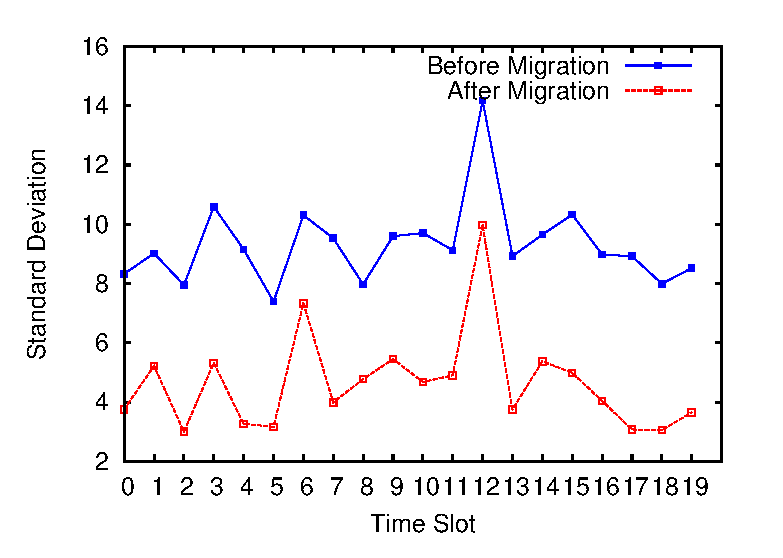
\includegraphics[width=\linewidth]{chap5/central.eps}
    \caption{Performance of Centralized Scheme}\label{central}
  \end{minipage}\hspace{0.3cm}
  \begin{minipage}[t]{0.45\textwidth}
    \centering
    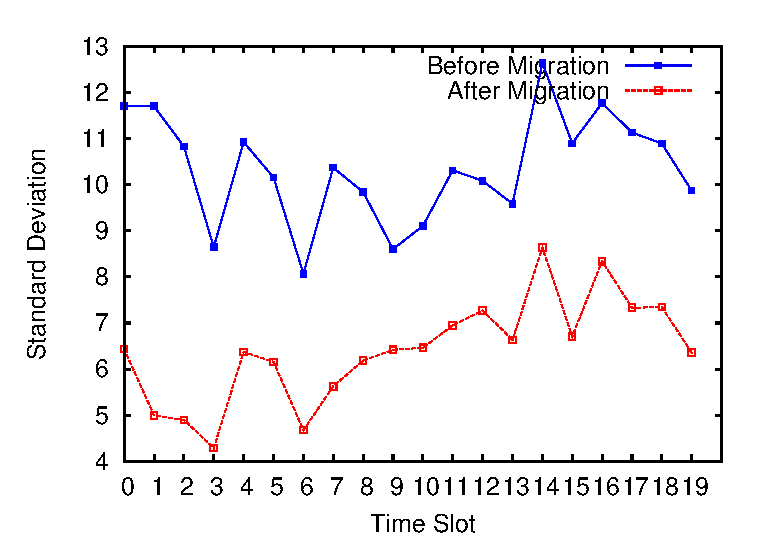
\includegraphics[width=\linewidth]{chap5/distribute.eps}
  \caption{Performance of Distributed Scheme}\label{distribute}
  \end{minipage}\hspace{0.3cm}
\end{figure}

From Figure ~\ref{central} and Figure ~\ref{distribute}, we can notice that, our LBMC schemes are effective. The weight of each switch obeys the Pareto Distribution with its parameter $\alpha=3$, and changes at different time slots. Then for both the NCM-LBMC scheme and the DM-LBMC scheme, the standard deviation decreases after the migration is done. This is because these two methods manages to move switches from overloaded controllers to idle controllers. And we can see that the performance of the naive centralized version is a little better than the distributed version. This is because the centralized controllers can get the information of the whole network, and make the best choices in the migrating process. Each switch may have a lot of destinations, and it is also possible to move a switch from controller $c_a$ to a controller $c_b$ that is very far from $c_a$. However, in the distributed version, the controllers can only get local information, and move switches to nearby controllers. This limits the scalibality of this load balancing scheme, and in this way, we make local-optimal choices instead of global-optimal choices.
\begin{figure}[!htbp]
\begin{minipage}[t]{0.45\textwidth}
    \centering
    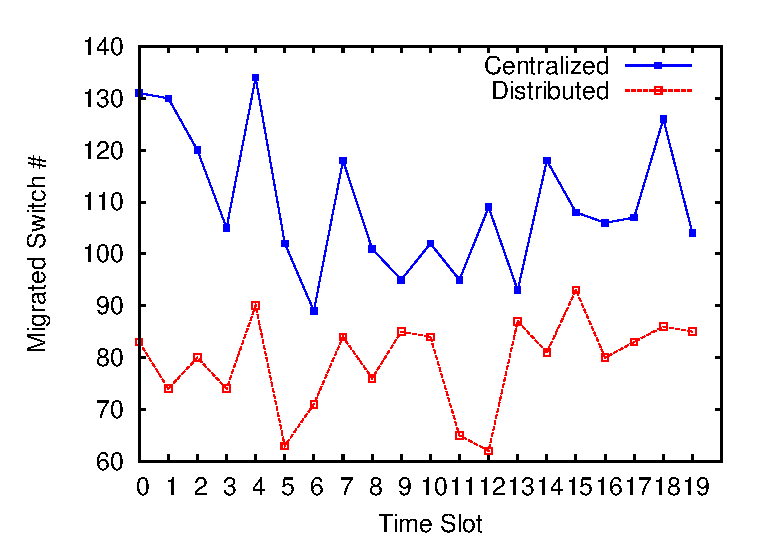
\includegraphics[width=\linewidth]{chap5/migswitch.eps}
    \caption{The Comparison of Migrated Switches}\label{migswitch}
  \end{minipage}\hspace{0.3cm}
  \begin{minipage}[t]{0.45\textwidth}
    \centering
    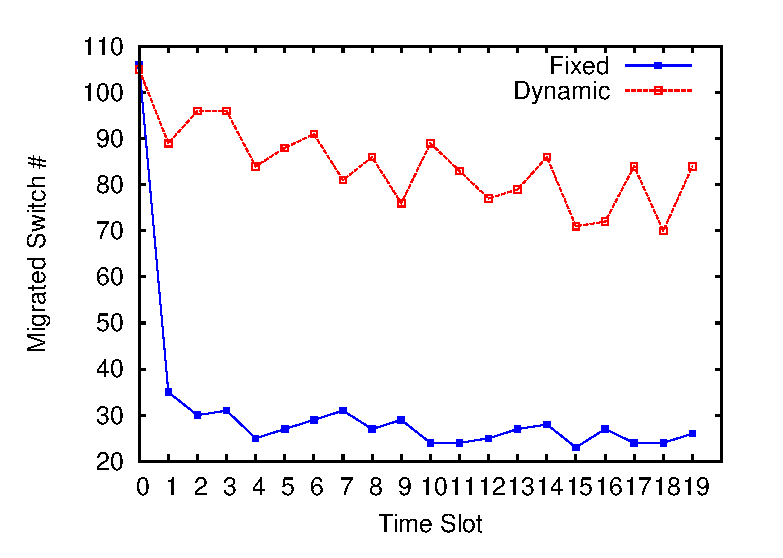
\includegraphics[width=\linewidth]{chap5/fixdynamic.eps}
    \caption{Migrated Switches of DM-LBMC}\label{fixdynamic}
  \end{minipage}\hspace{0.3cm}
\end{figure}

In Figure ~\ref{migswitch}, we notice that the number of migrated switches in the centralized scheme is larger than the number in the distributed scheme. This is also because the centralized version have a global view. Every time the load in the network changes, a switch can be moved to any of its reachable controllers. But in the distributed version, a switch can only be migrated to a controller that is the neighbor of the current one. And for local hot spots, this will prohibit the migrating phase. In this part, we compare the migrating switch number of NCM-LBMC and DM-LBMC in the condition that the whole weight in the network is changing, and we can see that the migrated switches at different time slot is nearly the same. And if the weight in the system is fixed, the centralized version still holds this feature since it has a global perspective, but the distributed version no more holds it. In Figure ~\ref{fixdynamic}, the number of migrated switches remains stable in conditions with dynamic total weight. If controller $c1$ is overloaded, it will send some switches to its nearby controllers. But if in the next round, the switches that monitored by those controllers gain higher traffic load and make the nearby controllers overloaded, then the switches may be sent back to controller $c1$. And if the total weight of the system is fixed, the number of migrated switches with decreases rapidly, and then holds stable. This is because DM-LBMC only migrates locally, and as the system becomes more balanced, the scheme will only need to move a few switches to make some micro adjustments. 

\vspace{-5pt}
\section{Different Centralized Schemes}

We then examine the performance of different kinds of centralized schemes. We modified the naive centralized load balancing scheme, and raise another two schemes: NCM-LBMC and SPCM-LBMC. These two schemes take the problem of capacity limits and system value into consideration.

\begin{figure}[!htbp]
\begin{minipage}[t]{0.45\textwidth}
    \centering
    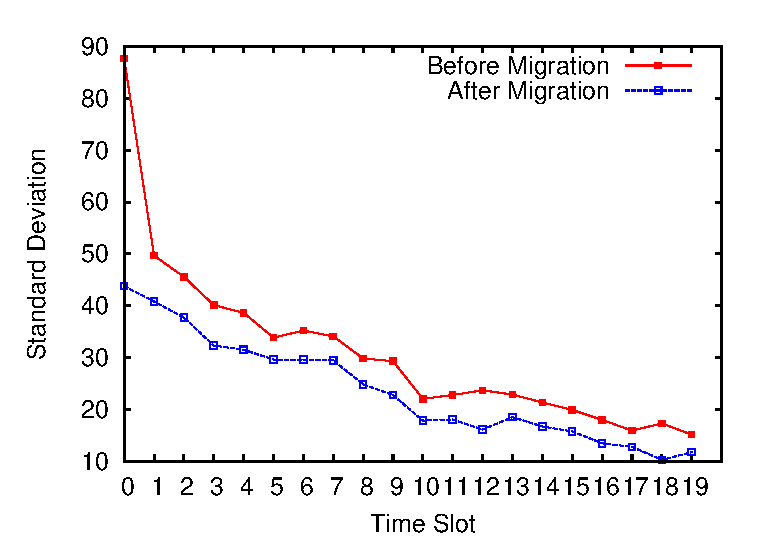
\includegraphics[width=\linewidth]{chap5/weightgraph.eps}
    \caption{Standard Deviation of limited CM-LBMC}\label{weightgraph}
  \end{minipage}\hspace{0.3cm}
  \begin{minipage}[t]{0.45\textwidth}
    \centering
    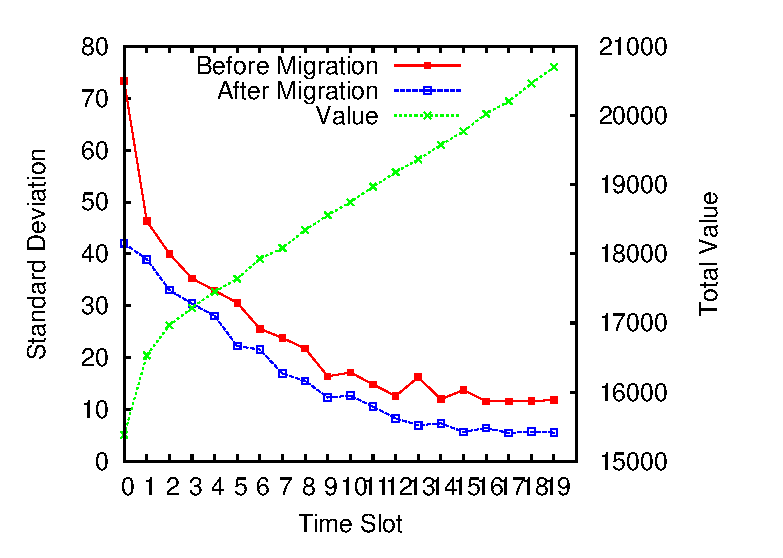
\includegraphics[width=\linewidth]{chap5/valuegraph.eps}
    \caption{Standard Deviation of Switch-Priority-based CM-LBMC}\label{valuegraph}
  \end{minipage}\hspace{0.3cm}
\end{figure}

Figure ~\ref{weightgraph} and Figure ~\ref{valuegraph} show the performance of these two modified algorithms. In limited CM-LBMC, the maximum performance of each controller also follows Pareto distribution with $\alpha=3$, and we amplify it with a constant to make sure the total traffic load not exceed the capacity of all controllers. In CM-LBMC with switch priority, we allocate a value to each mapping of a switch and a controller, which is inversely proportional to their distance. Fig. \ref{weightgraph} shows the standard deviation of our limited CM-LBMC at different time slots. We can see that the standard deviation is decreasing, but is still obviously higher than that in naive CM-LBMC. This is because in limited CM-LBMC, each controller has a different upper bound, this will influence the migration. For example, if some switches can only be monitored by a certain controller, and that controller is overloaded, then this will cause a high standard deviation since we cannot remove the switches to other controllers. It is similar in CM-LBMC with switch priority, which is shown in Figure \ref{valuegraph}. Meanwhile, in Figure \ref{valuegraph}, we show that the total value of the whole network is increasing, and the standard deviation is decreasing. And the standard deviation we get when it becomes stable is also acceptable. Thus, our schemes are effective and also practical.

%%==================================================
%% chapter03.tex for SJTU Bachelor Thesis
%% version: 0.5.2
%% Encoding: UTF-8
%%==================================================

% \bibliographystyle{sjtu2} %[此处用于每章都生产参考文献]

\chapter{Further Discussion}
\label{chap:discuss}

Then we make some further discussion on the LBMC problem. In the schemes we presented, we mainly devided the process into two phases: the initialization phase and the migration phase. In a DCN that deploys OpenFlow protocol, we only need to execute the initialization once, and then do migration periodically. The original schemes for controllers are naive, omitting the capacity of controllers and the value of the network. And we optimize these schemes to make them practical in real network environments. However, for the modified centralized schemes and the distributed schemes, there are still several problems to be solved in the future.

\textbf{Flexible controller number} : In our scheme, we use a fixed number of controllers to monitor the whole network. Furthermore, we suppose that all controllers in the network have to be used. However, in real applications, the total traffic in the network may be far less then the total capacity of all the controllers, i.e., the system can run in a good condition using only a part of the controllers. Thus, a new scheme can be deployed to modify the number of active controllers as the load changes. This can save the energy and also decrease the complexity of calculating balancing strategies. Related researches are also done in the elastic distributed controller architecture \cite{elasticsdn}.

\textbf{Hot controllers} : For a complex network, a controller may have a plenty of reachable switches. And in our SPCM-LBMC scheme, if the value of the link between this controller and its switches are high, this controller is very likely to become a hot spot in the end. Thus, to solve this problem, in future work, we intend to introduce a parameter to record the popularity of each controller. For those controller that has high popularity, we will decrease its link value to prevent it from being attached by many switches. Or we can define a probability according to  its popularity. Each switch obey this probability to connect to this controller. And if the popularity of the controllers are quite high, several controllers that have the same reachable switches as the hot controller can be added in the network to share its load.

\textbf{Mixed structures} : For real applications, it may be impractical to deploy our centralized algorithms since the delivery of global information may be very hard for large DCN. However, for distributed schemes, we will meet a trouble when some of the controllers are down. Since controllers in distributed schemes can only get information of its nearby region, the breakdown of some controllers will cause local hot spots that will take a long time to disappear. Thus, a mixed structure is needed to solve the dilemma. In the mixed strategy such as in \cite{kandoo}, the network is devided into several regions, and there will be a centralized controller to monitor all the distributed controllers in each region. Every time a distributed controller is down, its centralized controller will notify all other centralized controllers, and then the system will take a special scheme to share the load of the breakdown controller quickly. All centralized controllers are connected and will communicate once in a while. This hierarchical structure will make the management of distributed controllers effective and easy.

%%==================================================
%% chapter03.tex for SJTU Bachelor Thesis
%% version: 0.5.2
%% Encoding: UTF-8
%%==================================================

% \bibliographystyle{sjtu2} %[此处用于每章都生产参考文献]

\chapter{Related Works}
\label{chap:related}

Since the amount of data needed in real networks are dramatically increasing, tons of researches have been done to increase the efficiency of current DCNs \cite{dcnarch,hedera,spain,vl2,elastictree,flyways}. And in order to make the management of DCN effective and easy, several structures are also raised to deploy SDN in data centers, such as Global Environment for Network Innovations (GENI) of US, Future Internet Research and Experimentation Initative (FIRE) of EU, AKARI \& JGN2plus of Japan, and Smart Applications on Virtual Infrastructure (SAVI) of Canada. Among these works, OpenFlow is the most popular one, which uses software controllers to manipulate the whole system.

In early data centers that deploys such structures, a centralized controller is usually used to control the whole system. A DCN that uses a centralized controller is very easy to deploy, and also saves the energy of many controllers. \cite{hedera,spain,openflow,elastictree} are examples of this kind. They can get the global information of the network, and then make appropriate choices when flows come in. It is obvious that a centralized controller is enough for a data center that is not very large, and it also simplifies the process of making decisions.

Nevertheless, a simple centralized controller can also easily becomes the bottleneck of the whole system. When the DCN is very large and complex, the performance of the system will be influenced by the limited capacity of this single controller. Thus, researchers raised the idea of devolved controllers \cite{devolved,devolvedglobecom,elasticsdn,hyperflow,inpacket,multictr} to solve the problem of scalability. Using devolved controllers, the system will be split into several parts, and each devolved controller will work as a centralized controller in its own region.

At the same time, some other scholars also did some research \cite{localcen,elasticsdn,hyperflow,inpacket,onix} on distributed controllers for this SDN structure, to solve the problem of scalability in centralized structure. These researches discuss the statically configured and dynamically configured mapping between a switch and a controller in SDN. Software Defined Networking (SDN) enables the programmability of the network, and brings easier control and fantanstic innovation \cite{openflow,ethane,soft}. In SDN standard that specified by Open Networking Foundation \cite{onf}, the control plan and the data plane are seperated. Currently, one widely used protocol in SDN is OpenFlow \cite{openflow}, which is raised by Stanford University. In OpenFlow, the control plane can manipulate the flows in the data plane by using programmable controllers. And as we mentioned above, a single centralized controller will become the bottleneck of the system, thus works such as HyperFlow \cite{hyperflow}, DevoFlow \cite{DevoFlow}, DAIM \cite{DAIM} and Devolved Controllers \cite{devolved} are attempting to address this issue, by either using multiple controllers or devolving network control to switches. And all these methods requires a global view of the network. Comparatively, a hierarchical structure Kandoo \cite{kandoo} only needs local information in its bottom layer, and requires global information in its top layer.

Except for these theoretical researches, may works are done in practical area. Authors in \cite{DOT} present a low cost network emulator called Distributed OpenFlow Testbed (DOT), which can emulate large SDN deployments, thus making it convenient for scholars to test their schemes. And Google also published their B4 \cite{B4} network, which is established on a DCN that is based on OpenFlow. B4 is devided into three layers: switch hardware layer, site controllers layer and global layer. Each site is a data center in B4. The switches and controllers are deployed in every data center, while the SDN gateway and the Traffic Engineering (TE) servers are deployed in a centralized area. Another migration protocol based on OpenFlow is presented by the authors in \cite{elasticsdn}. By all these achievements above, the commercialized ultilization of OpenFlow is currently on its right track.

%%==================================================
%% conclusion.tex for SJTU Bachelor Thesis
%% version: 0.5.2
%% Encoding: UTF-8
%%==================================================

\chapter{Conclusion}
\label{chap:conclusion}

With the impressive development of the scale of DCN, it becomes very hard to use a centralized controller to manipulate the traffic flows in a DCN that deploys the OpenFlow protocol, thus leading to overloaded controllers and reduce the performance of the network. The emergence of devolved controllers provides us with innovate methods to address this scalability issue. In this paper, we use multiple controllers to solve the problem of load balancing. First we define the Load Balancing problem of Multiple Controllers (LBMC), and analyse the necessary conditions to solve this problem in real applications. Then we give the naive centralized migration scheme and the distributed migration scheme, where controllers have no limits. However, in real world environments, each controller has a capacity limit, and switches may also have different priorities. Thus we established a load balancing model with capacity limits and values of OpenFlow network, and raised an algorithm to maximize the value as well as minimize the difference on ultilization ratio. By implementing all above algorthms and doing simulations, we prove the effectiveness of the algorithms, and also prove the possibity of deploying these algorithms in real software defined networks. This paper is inspired by several works of predecessors, and manages to optimize their schemes for real applications. We finally present several optimizations that can be done in the future to improve the performance of our algorithms. 
 %% 全文总结


%%%%%%%%%%%%%%%%%%%%%%%%%%%%%% 
%% 附录(章节编号重新计算,使用字母进行编号)
%%%%%%%%%%%%%%%%%%%%%%%%%%%%%% 
\appendix

% 附录中编号形式是"A-1"的样子
\renewcommand\theequation{\Alph{chapter}--\arabic{equation}}
\renewcommand\thefigure{\Alph{chapter}--\arabic{figure}}
\renewcommand\thetable{\Alph{chapter}--\arabic{table}}

%\include{body/app1} % 更新记录
%\include{body/app2} % 麦克斯韦方程
% \include{body/app3}


%%%%%%%%%%%%%%%%%%%%%%%%%%%%%% 
%% 文后(无章节编号)
%%%%%%%%%%%%%%%%%%%%%%%%%%%%%% 
\backmatter

% 参考文献
% 使用 BibTeX
% 包含参考文献文件.bib
\begin{thebibliography}{1}
\bibitem{geni} ``Global Environment for Network Innovations(GENI).'' [Online Website]. Available: http://www.geni.net/
\bibitem{fire} ``Future Internet Research and Experimentation Initative(FIRE).'' [Online Website]. Available: http://cordis.europa.eu/fp7/ict/fire/
\bibitem{akari} ``AKARI \& JGN2plus.'' [Online Website]. Available: http://www.nict.go.jp/en/photonic\_nw/archi/akari/akari-top\_e.html
\bibitem{savi} ``Smart Applications on Virtual Infrastructure(SAVI).'' [Online Website]. Available: http://www.savinetwork.ca/
\bibitem{openflow}N. McKeown, T. Anderson, H. Balakrishnan, et al. ``OpenFlow: enabling innovation in campus networks,'' \emph{ACM SIGCOMM}, 69-74, 2008.
\bibitem{ethane} M. Casado, M. J. Freedman, and S. Shenker, ``Ethane: Taking Control of the Enterprise,'' \emph{ACM SIGCOMM}, 2007.
\bibitem{sane} ``Clean-Slate Security Architecture (SANE).'' [Online Website]. Available: http://www.geni.net/
\bibitem{4d1} A. Greenberg, G. Hjalmtysson, D. A. Maltz, et al., ``Refactoring network control and management: A case for the 4D architecture ,'' tech. rep., Computer Science Department, Carnegie Mellon University, 2005.
\bibitem{4d2} A. Greenberg, G. Hjalmtysson, D. A. Maltz, et al., ``A clean slate 4D approach to netw ork control and management,'' \emph{SIGCOMM CCR}, 2005.
\bibitem{openbook}S. Azodolmolky, ``Software Defined Networking with OpenFlow,'' Packt Publishing Ltd., 2013.
\bibitem{devolved}AS-W. Tam, K. Xi, and H. Chao. ``Use of devolved controllers in data center networks." \emph{IEEE INFOCOM}, 596-601, 2011.
\bibitem{devolvedglobecom}AS-W. Tam, K. Xi, and H. Chao. ``Scalability and Resilience in Data Center Networks: Dynamic Flow Reroute as an Example,'' \emph{IEEE GLOBECOM}, 1-6, 2011.
\bibitem{multictr}Li Y, Dong L, Qu J, et al. ``Multiple controller management in software defined networking,''\emph{SCAC},2014.
\bibitem{elasticsdn}A. Dixit, F. Hao, et al. ``Towards an elastic distributed sdn controller." \emph{ACM SIGCOMM}, 7-12, 2013.
\bibitem{lwc}W. Liang, X. Gao, F. Wu, et al., ``Balancing traffic load for devolved controllers in data center networks,'' \emph{GLOBECOM}, 2258-2263, 2014.
\bibitem{localcen}D. Levin, A.Wundsam, B. Heller, et al. ``Logically centralized?: state distribution trade-offs in software defined networks,''ACM the first workshop on Hot topics in Software Defined Networks (HotSDN), 1-6, 2012.
\bibitem{dcnarch}M. Al-Fares, A. Loukissas, and A. Vahdat. ``A scalable, commodity data center network architecture,'' \emph{ACM SIGCOMM}, 63-74, 2008.
\bibitem{onf} ``Open Networking Foundation (ONF),'' [Online Website]. Available: http://www.opennetworking.org/
\bibitem{opproto} Open Networking Foundation, ``OpenFlow Switch Specification (Version 1.3.0),'' June 2012.
\bibitem{ryu} ``Ryu SDN Framework,'' [Online Website]. Available: http://osrg.github.io/ryu/
\bibitem{kandoo}S. Yeganeh and Y. Ganjali. ``Kandoo: a framework for efficient and scalable offloading of control applications." \emph{ACM HotSDN}, 19-24, 2012.
\bibitem{hedera}M. Al-Fares, S. Radhakrishnan, et al. ``Hedera: Dynamic flow scheduling for data center networks,'' \emph{USENIX NSDI},19-19, 2010.
\bibitem{spain}J. Mudigonda, et al. ``SPAIN: COTS Data-Center Ethernet for Multipathing over Arbitrary Topologies." \emph{USENIX NSDI}, 265-280, 2010.
\bibitem{vl2}A. Greenberg, J. Hamilton, N. Jain, et al. ``VL2: a scalable and flexible data center network,'' \emph{ACM SIGCOMM}, 51-62, 2009.
\bibitem{elastictree}B. Heller, S. Seetharaman, et al. ``ElasticTree: Saving Energy in Data Center Networks'' \emph{USENIX NSDI}, 249-264, 2010.
\bibitem{flyways}S. Kandula, J. Padhye, and P. Bahl. ``Flyways to de-congest data center networks." \emph{ACM Hotnets-VIII}, 2009.
\bibitem{hyperflow}A. Tootoonchian, Y. Ganjali. ``HyperFlow: A distributed control plane for OpenFlow." \emph{USENIX INM/WREN}, 3-3, 2010.
\bibitem{inpacket}C. Macapuna, C. Rothenberg, M. Magalhaes. ``In-packet Bloom filter based data center networking with distributed OpenFlow controllers." \emph{IEEE GLOBECOM}, 584-588, 2010.
\bibitem{onix}T. Koponen, et al. ``Onix: A Distributed Control Platform for Large-scale Production Networks." \emph{USENIX NSDI}, 1-6, 2010.
\bibitem{soft}T. V.Lakshman, et al. ``The softrouter architecture,'' \emph{Proc. ACM SIGCOMM Workshop on Hot Topics in Networking}, vol. 2004, 2004.
\bibitem{DevoFlow} Curtis, Andrew R., et al. ``DevoFlow: Scaling flow management for high-performance networks.'' ACM SIGCOMM Computer Communication Review, 254-265, 2011.
\bibitem{DAIM} Banjar, Ameen, Pakawat Pupatwibuli, and Robin Braun. ``DAIM: a mechanism to distribute control functions within OpenFlow switches.'' \emph{Journal of Networks}, 1-9, 2014.
\bibitem{DOT} Roy, Arup Raton, et al. ``Design and management of dot: A distributed openflow testbed.'' Network Operations and Management Symposium (NOMS), 2014.
\bibitem{B4} S. Jain and al., ``B4: Experience with a Globally-Deployed Software Defined WAN,'' ACM International Conference on the applications, technologies, architectures, and protocols for computer communication (SIGCOMM), 2013.
\end{thebibliography}

%% 个人简历(学士学位论文没有个人简历要求)
% %%==================================================
%% resume.tex for SJTU Bachelor Thesis
%% version: 0.5.2
%% Encoding: UTF-8
%%==================================================

\begin{resume}

\begin{resumesection}{基本情况}
xxx,男,上海人,19XX 年~XX 月出生,未婚,
上海交通大学XX系在读。
\end{resumesection}

\begin{resumelist}{教育状况}
XXXX 年~9 月至~XXXX 年~7 月,上海交通大学, 本科,专业:XXXX

XXXX 年~9 月至~XXXX 年~7 月,上海交通大学, 硕士研究生,专业:XXXX

XXXX 年~9 月至~XXXX 年~7 月,上海交通大学,
博士研究生(提前攻读博士),专业:XXXX
\end{resumelist}

\begin{resumelist}{工作经历}
无。
\end{resumelist}

\begin{resumelist}{研究兴趣}
XXXXXXX。
\end{resumelist}

\begin{resumelist}{联系方式}
通讯地址:上海市闵行区东川路800号,上海交通大学

邮编:200240

E-mail: abcde@sjtu.edu.cn
\end{resumelist}

\end{resume}


% 致谢
%%==================================================
%% thanks.tex for SJTU Bachelor Thesis
%% version: 0.5.2
%% Encoding: UTF-8
%%==================================================

\begin{thanks}

Here, I sincerely express my gratitude to all those who have ever helped me to accomplish this topic during my last few months in Shanghai Jiao Tong University. The selfless and enthusiasim of them really helps a lot in my algorithm designing part and my evalution part. 

Firstly, I have to appreciate my supervisor, Professor Xiaofeng Gao, for her valuable advices and selfless assistance in the whole process. From the beginning stage, she gave me many suggestions on my topic, and taught me how to make innovations in this area. She also led me to the world of doing rigorous researches. With her help, I learnt how to establish a model and analyse its complexity. I also learnt how to design acceptable and practical algorithms and test them by doing simulation. It was her that guided me a lot in this world of computer network, and gave me confidence to proceed my topic on OpenFlow. She is the most important person for me to finish my graduation project.

Then, I am very thankful to Mr. Wanchao Liang, who is a pioneer in the area of load balancing in DCN in our lab. It was based on his previous work that I further my research. He also instructed me how to do in some key stage. Without his effort, I would not be able to perfect the load balancing schemes in OpenFlow. I appreciate it a lot for his assistance in establishing the model, and I wish him a bright future.

Finally, I would send my thanks to Professor Guihai Chen and all my friends and schoolmates who have taken effort on this draft. Some of them helps me make a lot progress in the evaluation part, and some of them cheers me up when I confront difficulties in this project. Thanks for my classmates in the IEEE class, who inspire me to take actions to improve myself. And also thanks for ANL for the environent it provided for all these two years, which improves my ability during my undergraduate days.

\end{thanks}



% 发表文章目录
%%%==================================================
%% pub.tex for SJTU Bachelor Thesis
%% version: 0.5.2
%% Encoding: UTF-8
%%==================================================

\begin{publications}{99}

    \item\textsc{Chen H, Chan C~T}. {Acoustic cloaking in three dimensions using acoustic metamaterials}[J].
      Applied Physics Letters, 2007, 91:183518.

    \item\textsc{Chen H, Wu B~I, Zhang B}, et al. {Electromagnetic Wave Interactions with a Metamaterial Cloak}[J].
      Physical Review Letters, 2007, 99(6):63903.
    
\end{publications}


% 参与项目列表
%%%==================================================
%% projects.tex for SJTU Bachelor Thesis
%% version: 0.5.2
%% Encoding: UTF-8
%%==================================================

\begin{projects}{99}

    \item 973项目“XXX”
    \item 自然基金项目“XXX”
    \item 国防项目“XXX”
    
\end{projects}


%英文大摘要
%\include{body/bigabstract}

\end{document}
